%Preamble--------------------------------------------------------------------------------------------

\documentclass[11pt,a4paper,twoside,openright]{report}

\usepackage[ top=30mm, bottom=20mm ]{geometry} %This package lets you specify the margin widths.

\usepackage{textcomp} %This package formats the greek symbol mu properly.

\usepackage[round,authoryear]{natbib} %This package is to make nice author date citations.
\renewcommand\cite{\citep} %in the natlab package cite is citep so change command to cite.
\renewcommand{\bibname}{References} %This is make the bibliography be called references.

\usepackage{lscape} %This package is meant to let you turn a single page into a landscape view by writing the section in the landscape environment.

\usepackage{tabularx} %This package makes writing tables easier. It does some magic with the column widths.
\usepackage{booktabs} %This package allows some more fancy formatting with tables such as thicker header lines.
\usepackage{pdfpages} %This package is meant to let you insert multiple pdf page into your latex document.

\usepackage[hidelinks]{hyperref} %this package makes hyperlinks between citations and figures and the body of the text.
\newcommand{\figref}[1]{(\autoref{#1})} %this command will correctly name a figure reference, surround with parentheses and make it a clickable link.
\newcommand{\tabref}[1]{(\autoref{#1})} %this command will correctly name a table reference, surround with parentheses and make it a clickable link.

\usepackage[all]{hypcap} %This package should make it so that when you click on a link to a table or figure, the page is oriented to the figure/table, not the the caption.

\usepackage{setspace} %this package is to set the line space easily
\onehalfspacing %set to one and a half spacing

\usepackage[printonlyused]{acronym} %This package helps manage a list of acronyms
\usepackage{relsize} %This package supports the acronym package by making the acronyms appear smaller in the text.

\usepackage{graphicx} %This is some package for including figures images.

\usepackage{url} %This package helps format the urls over the line breaks.


%End-preamble----------------------------------------------------------------------------------------

\begin{document}

%Frontmatter-----------------------------------------------------------------------------------------

% Thesis/dissertation sheet goes in the inside cover of the thesis. This doc contains the abstract

\includepdf{abstract_figures/thesisdissertation_SY.pdf}
\newpage


%Title page
 %Title page
\begin{titlepage}
\begin{center}
\vspace*{1in}
\LARGE{\textbf{Molecular microbial ecology of Antarctic lakes}}
\par
\vspace{1.5in}
\LARGE{Sheree Yau}
\vfill
\par
\normalsize{A thesis in fulfilment of the requirements for the degree of Doctor of Philosophy}
\par
\vspace{0.5in}
\normalsize{School of Biotechnology and Biomolecular Sciences}
\par
\normalsize{Faculty of Science}
\par
\large{University of New South Wales, Australia}
\par
\vspace{0.5in}
\normalsize{February, 2013}
\par
\vspace{0.5in}
\end{center}
\end{titlepage}


%number the front matter with roman numerals
\pagenumbering{roman}

\chapter*{Originality Statement}
%\addcontentsline{toc}{chapter}{Originality Statement}
`I hereby declare that this submission is my own work and to the best of my knowledge it contains
 no materials previously published of written by another person, or substantial proportions of 
material which have been accepted for the award of any other degree or diploma at UNSW or any other
 educational institution, except where due acknowledgement is made in the thesis. Any contribution 
made to the research by others, with whom I have worked at UNSW or elsewhere, is explicitly 
acknowledged in the thesis. I also declare that the intellectual content of this thesis is the product
 of my own work, except to the extent that assistance from others in the project's design and 
conception or in style, presentation and linguistic expression is acknowledged.'\\\\
Signed \dotfill\\\\
Date \dotfill

%\include{copyright}
\chapter*{Authenticity statement}
\addcontentsline{toc}{chapter}{Authenticity statement}
`I certify that the Library deposit digital copy is a direct equivalent of the final officially approved version of my thesis.
No emendation of content has occurred and if there are any minor variations in formatting, they are the result of the conversion to digital format.'

\chapter*{Acknowledgements}
%\addcontentsline{toc}{chapter}{Acknowledgements}
\newpage

\chapter*{List of Publications}
%\addcontentsline{toc}{chapter}{List of Publications}
Publications and submitted manuscripts arising from my PhD research are listed below.
In all cases, my supervisor Prof Ricardo Cavicchioli and my co-supervisor Dr Federico Lauro were
involved in the research design and editing of the manuscripts.
Where versions of published material, or material submitted for publication appears in this thesis, details of the contributions made by myself and others precede it.

\begin{itemize}

\item \textbf{Sheree Yau}, Federico M. Lauro, Timothy J. Williams, Matthew Z. DeMaere, Mark V. Brown, John Rich, John A.E. Gibson, Ricardo Cavicchioli. 
Strategies of carbon conservation and unusual sulfur biogeochemistry in a hypersaline lake.
\emph{\underline{ISME Journal}}
(submitted), 2013.

\item Khawar S. Siddhiqui, Timothy J. Williams, David Wilkins, \textbf{Sheree Yau}, Michelle A. Allen, Mark V. Brown, Federico M. Lauro, Ricardo Cavicchioli.
Psychrophiles.
\emph{\underline{Annual Review of Earth and Planetary Sciences}}
(in press), 2013.

\item David Wilkins, \textbf{Sheree Yau}, Timothy J. Williams, Michelle Allen, Mark V. Brown, Matthew Z. DeMaere, Federico M. Lauro and Ricardo Cavicchioli.
Key Microbial Drivers in Antarctic Aquatic Environments.
\emph{\underline{FEMS Microbiology Reviews}}
(10.1111/1574-6976.12007), 2012.

\item \textbf{Sheree Yau} and Ricardo Cavicchioli. 
Microbial communities in Antarctic lakes: Entirely new perspectives from metagenomics and metaproteomics. 
\emph{\underline{Microbiology }}
\emph{\underline{Australia}} 32:157--159, 2011.

\item Federico M. Lauro, Matthew Z. DeMaere, \textbf{Sheree Yau}, Mark V. Brown, Charmaine Ng, David Wilkins, Mark J. Raftery, John A.E. Gibson, Cynthia Andrews-Pfannkoch, Matthew Lewis, Jeffery M. Hoffman,Torsten Thomas and Ricardo Cavicchioli. 
An integrative study of a meromictic lake ecosystem in Antarctica. 
\emph{\underline{ISME Journal}}
5:879--895, 2011.

\item \textbf{Sheree Yau}, Federico M. Lauro, Matthew Z. DeMaere, Mark V. Brown, Torsten Thomas, 
Mark J. Raftery, Cynthia Andrews-Pfannkoch, Matthew Lewis, Jeffery M. Hoffman, John A. Gibson and 
Ricardo Cavicchioli. 
Virophage control of antarctic algal host--virus dynamics. 
\emph{\underline{Proceedings of the National Academy of Sciences}}
\emph{\underline{USA}} 108:6163--6168, 2011.

\end{itemize}



\tableofcontents
\listoffigures
\listoftables
\chapter*{List of Abbreviations}

\begin{acronym}

\acro{1D-SDS PAGE}{one dimensional-sodium dodecyl sulphate polyacrylamide gel electrophoresis}

\acro{2D-SDS PAGE}{two dimensional-sodium dodecyl sulphate polyacrylamide gel electrophoresis}

\acro{AAnP}{aerobic anoxygenic photosynthesis}

\acro{ABC}{ATP-binding cassette}

\acro{ANOSIM}{analysis of similarity}

\acro{APMV}{\emph{Acanthamoeba polyphaga} mimivirus}

\acro{BchlA}{bacteriochlorophyll A}

\acro{BLAST}{basic local alignment search tool}

\acro{C-ace}{green sulphur bacteria from Ace Lake related to \emph{Chlorobium}}

\acro{CAMERA}{Community Cyberinfrastructure for Advanced Microbial Ecology Research and Analysis}

\acro{CAS}{CRISPR-associated proteins}

\acro{COG}{clusters of orthologous groups}

\acro{CRISPR}{clustered regularly interspaced short palindromic repeat}

\acro{DGGE}{denaturing gradient gel electrophoresis}

\acro{DMS}{dimethylsulphide}

\acro{DMSO}{dimethylsulphoxide}

\acro{DMSP}{dimethylsulphoproprionate}

\acro{DNA}{deoxyribonucleic acid}

\acro{DPOB}{DNA polymerase B}

\acro{DO}{dissolved oxygen}

\acro{DOC}{dissolved organic carbon}

\acro{DRP}{dissolved reactive phosphorus}

\acro{GOS}{global ocean sampling}

\acro{GSB}{green sulphur bacteria}

\acro{HMMER}{biosequence analysis using profile hidden Markov models}

\acro{JCVI}{J.Craig Venter Institute}

\acro{KEGG}{Kyoto Encyclopedia of Genes and Genomes}

\acro{KO}{KEGG Orthology}

\acro{KOBAS}{KEGG Orthology Based Annotation System}

\acro{MCP}{major capsid protein}

\acro{MS}{mass spectrometry}

\acro{MS-MS}{two dimensional mass spectrometry}

\acro{NCBI}{National Center for Biotechnology Information}

\acro{NR}{non-redundant database}

\acro{OLPV}{Organic Lake phycodnavirus}
\acrodefplural{OLPV}{Organic Lake phycodnaviruses}

\acro{ORF}{open-reading frame}

\acro{OTU}{operational taxonomic unit}

\acro{PCA}{Principal Component Analysis}

\acro{PCR}{polymerase chain reaction}

\acro{PCTE}{polycarbonate Track Etch$^{TM}$}

\acro{POC}{particulate organic carbon}

\acro{PR}{proteorhodopsin}

\acro{PV}{phycodnavirus}
\acrodefplural{PV}{phycodnaviruses}

\acro{QIIME}{Quanititative Insights Into Microbial Ecology}

\acro{RDP}{Ribosomal Database Project}

\acro{RNA}{ribonucleic acid}

\acro{rRNA}{ribosomal RNA}

\acro{rTCA}{reverse tricarboxylic acid}

\acro{RuBisCO}{ribulose-bisphosphate carboxylase oxygenase}

\acro{SDS}{sodium dodecyl sulphate}

\acro{SDS PAGE}{sodium dodecyl sulphate-polyacrylamide gel electrophoresis}

\acro{SO}{Southern Ocean}

\acro{SRB}{sulphate-reducing bacteria}

\acro{SRP}{soluble reactive phosphate}

\acro{SSU}{small subunit ribosomal RNA}

\acro{STAMP}{Statistical Analysis of Metagenomic Profiles}

\acro{TEM}{transmission electron microscopy}

\acro{TDN}{total dissolved nitrogen}

\acro{TDP}{total dissolved phosphorus}

\acro{TDS}{total dissolved sulphur}

\acro{TIGRFAM}{the Institute of Genomic Research curated protein database}

\acro{TN}{total nitrogen}

\acro{TOC}{total organic carbon}

\acro{TP}{total phosphorus}

\acro{TS}{total sulphur}

\acro{VLP}{virus-like particle}

\acro{WGS}{whole genome shotgun}

\acro{WL}{Wood-Ljungdahl; or reductive acetyl-CoA}

\end{acronym}


%End-frontmatter-------------------------------------------------------------------------------------

%Mainmatter-----------------------------------------------------------------------------------------

%Number the main text in arabic numerals
\pagenumbering{arabic}

\chapter[General Introduction]{General introduction: molecular microbial ecology of Antarctic lakes}
\label{ch:intro}

\section{Introduction}
Antarctica is a ``frozen desert'' of constant low temperature, little precipitation and long polar light cycles where only specially adapted organisms can survive.
Only 0.4\% of the total ice area of Antarctica (12.3 $\times$ 10$^6$ km$^2$) is seasonally ice-free, comprising exposed mountains and coastal areas. %ref
Life is concentrated on the few ice-free coastal oases where liquid water is present in hundreds of lakes and ponds.
Lake biota is microbially dominated with few or no metazoans present \cite{Laybourne-Parry1997}.
The reduced complexity means it is possible to encompass a large proportion of the diversity present through the use of molecular-based techniques.
The lakes inhabit a continuum of environmental factors, presenting themselves as ``natural laboratories'' where comparisons can be made between lakes that vary in a property of interest. 
Meromictic lakes similarly provide an opportunity to describe microbial populations along chemical gradients, but within a single water body. 
This makes Antarctic lakes ideal model ecosystems to examine microbial influence on geochemistry by relating taxa to particular processes\cite{Laybourne-Parry2007}.

This introduction will describe the Antarctic lakes, their microbiology and review the molecular-based microbiological research that has been conducted on the lakes.
As this thesis focused on two lakes in the Vestfold Hills, more emphasis will be given to describing research from this study site.

\section[Antarctic coastal oases]{Antarctic coastal oases and glacial lakes}
In Antarctica, perenially available liquid water is confined to coastal lakes, subglacial and epiglacial lakes.
Subglacial and epiglacial lakes appear to be prevalent with at least 145 subglacial lakes identified \cite{Siegert2005}.%check (Gibson, 2006; Cavicchioli, 2007; Pearce, 2009)
These include the largest, Lake Vostok. %name them.
Epiglacial lakes are. %describe them.

Coastal oases, where lakes are found exposed on the rocky land, include the Vestfold Hills, Bunger Hills, Larsemann Hills, Syowa Oasis, Schirmacher Oasis, Grearson Hills and McMurdo Dry Valleys
 in East Antarctica, the West Antarctic Peninsula and the sub-antarctic islands.
As Ad\'{e}lie penguins create nests from rocks, these few coastal oases are the only locations on the continent where they are able to breed.

Antarctic lakes span a wide range of physical and chemical properties from freshwater to hypersaline, ice-covered to perenially melted and permanently stratified (meromictic) to mixed (holomictic).
Most lakes are largely isolated due to long periods of ice-cover, and may be truly closed systems if ice-cover is permanent.
The age of water varies considerably, with the subglacial outflow from Blood Falls estimated to be 1.5 million years old \cite{Mickucki2009}, the water in Ace Lake about 5000 years old
 \cite{Rankin1999}, and Lake Miers water less than 300 years old \cite{Green1988}. %consider removing lake Miers. 
Organisms inhabiting the lakes may be examples of ancient life or undiscovered endemic species.

Of these locations, the best studied lake systems are those of the McMurdo Dry Valleys, The Vestfold Hills and the subantarctic islands.
%refer to table or map of the region
%How long have people done research on these lakes?


\section[Vestfold Hills]{The Vestfold Hills, East Antarctica}

The Vestfold Hills is a rocky ice-free region of approximately 400 km$^2$ on the eastern shore of the Prydz Bay, East Antarctica in the Australian Antarctic Territory (fig:vestfold map) \cite{Gibson1999}.
The region was first sighted and named in 1935\cite{Law1959}.
Only intermittent expeditions occurred in the area until the establishment of Davis Station (68$^{\circ}$33'S, 78$^{\circ}$15'E) in 1957 \cite {Law1959}. 
There Vestfold Hills region was immediately noted for its extensize ice-free land and the numerous lakes.\cite{Johnstone1973}.

The Australian Antarctic Data Centre lists more than 3000 water bodies mapped in the Vestfold Hills, ranging in area from 1 to 8,757,944 m\^{}2.%check this fact.
More than 300 lakes and ponds have been described, including approximately 20\% of the world's meromictic lakes \cite{Gibson, 1999}. %check this fact.
Fjords connected to the ocean also cut across the Vestfold Hills. 
Some of these are large, such as Ellis Fjord which is 10 km long, up to 100 m deep and has become a stratified system due to its restricted opening to the ocean \cite{Burke1988}.
The region was formed approximately 10,000 years ago when the retreat of the continental ice-shelf lead to isostatic uplift of the land \cite{Burton1981}. 

The lakes origated from water trapped in the exposed rocky depressions.
Many of the coastal lakes are marine-derived, having been separated from the marine environment 3,000--7,000 years ago \cite{Gibson1999} and are predominantly saline or hypersaline \cite{Burke1988}.
The latter are formed due to concentrated by ablation (evaporation and sublimnation). %ref 
Freshwater lakes near the continental ice shelf were likely already above sea-level as the ice receded and are not marine-derived \cite{Laybourne-Parry1992} \cite{Bronge1996}.
Lakes closer to the coast, such as Rookery Lake, may still occasionally experience marine inputs although most have completely separated from the sea. %ref

All lakes may receive water inputs from precipitation, from the ice-shelf and glacial melt streams \cite{Burton1981}. 
This can cause freshwater to seasonaly overlay some saline lakes as the ice-cover thaws.
Glacial meltwater flushing has lead some lakes that were originally marine-derived, such as Clear Lake, to become fresh \cite{Pickard1986}\cite{Bird1991}.
%Show a map of some of the main lakes in the Vestfold Hills
%Nutrient status? (see Burton 1981) temperature? weather? major ions? (see Burton1981). recorders of climate change in the sediment and in the location of the chemocline,what occurs in each zone
Since their formation each lake has followed a separate physical evolution depending on the local geography and now have very different chemical and physical properties. 

\subsection{Biology of the Vestfold Hills}

\subsection{Limnology of lakes of the Vestfold Hills}

Much early work was dedicated to the biology of the Vestfold Hills.
What was interesting and special?
What was the picture they had a microbial life?

\section[Antarctic microbiology]{Cultivation-based Antarctic microbiology}

Early microbiological surveys began X.
Bacteria were detected by cultivation or by microscopy. 
Identification was limited to those species that could be isolated and appropriate identification tests performed.
Eucarya were identified with microscopy based approaches.


\subsection{Eucarya}
\subsection{Bacteria}
\subsection{Archaea}
\subsection{Viruses}

\section{Molecular insights into Antarctic lakes}
\label{in:mol}
The majority of molecular-based studies of Antarctic aquatic microbial communities have made use of PCR amplification of small subunit ribosomal RNA sequences to survey the diversity of Bacteria
 and in some cases Archaea and Eucarya. %table
Microbial composition has been determined by cloning and sequencing of rRNA gene amplicons exclusively 
\cite{Bowman2000a, Bowman2000, Gordon2000, Christner2001, Purdy2003, Karr2006, Matsuzaki2006, Kurosawa2010,Bielewicz2011}, 
although most studies have also made use of denaturing gradient gel electrophoresis (DGGE) to provide a molecular ``fingerprint'' of the community 
\cite{Pearce2003, Pearce2003, Karr2005, Pearce2005, Pearce2005, Unrein2005, Glatz2006, Mikucki2007, Mosier2007, Schiaffino2009, Villaescusa2010}.
Functional genes have also been targeted using PCR amplification to assess the potential of biochemical processes occurring, such as nitrogen fixation \cite{Olsen1998}, 
ammonia oxidation \cite{Voytek1999}, anoxygenic photosynthesis \cite{Karr2003}, and dissimilatory sulfite reduction \cite{Karr2005, Mikucki2009}. %add in new studies

\section[Antarctic molecular studies]{Insights from Antarctic molecular studies}

\subsection{Bacterial diversity}
The vast majority of molecular studies of Antarctic lakes have focused on bacteria.
Consistent with the wide range of physical and chemical properties of Antarctic lakes, a large variation in species assemblages have been found.
While exchange of microorganisms must be able to occur between lakes that are in close vicinity to each other, 
the picture that has emerged from the data to date is that microbial populations are relatively unique to each type of isolated system. 
Nonetheless, certain trends in bacterial composition are also apparent.

\subsection{Bacterial diversity varies with salinity}
Focusing on the similarities, lakes of equivalent salinities tend to have similar communities.
Hypersaline lakes from the Vestfold Hills \cite{Bowman2000b} and McMurdo Dry Valleys \cite{Glatz2006, Mosier2007} were all dominated by Gammaproteobacteria and members of the Bacteroidetes
 as well as harboring lower abundance populations of Alphaproteobacteria, Actinobacteria, and Firmicutes.
The surface waters of saline lakes resemble marine communities dominated by Bacteroidetes, Alphaproteobacteria and Gammaproteobacteria,
 but divisions such as Actinobacteria and specific clades of Cyanobacteria have been found to be overrepresented compared to the ocean \cite{Lauro2011}.
Sediments from saline lakes in the Vestfold Hills \cite{Bowman2000a} and Nuramake-Ike in the Syowa Oasis \cite{Kurasawa2010} were very similar, 
containing in addition to the surface clades, Deltaproteobacteria, Planctomycetes, Spirochaetes, Chloroflexi (green non-sulfur bacteria), Verrucomicrobia and representatives of candidate divisions.
Plankton from freshwater lakes were characterized by an abundance of Betaproteobacteria, 
although Actinobacteria, Bacteroidetes, Alphaproteobacteria and Cyanobacteria were also prominent \cite{Pearce2003, Pearce2005, Pearce2005, Schiaffino2009}. 

\subsection{Bacterial diversity defined by nutrients}
Differences in bacterial community structure are also influenced by nutrient availability.
In studies of freshwater lakes in the Antarctic Peninsula and the South Shetland Islands, cluster analysis of DGGE profiles grouped together lakes of similar trophic status 
\cite{Schiaffino2009, Villaescusa2010}.
Most of the variance in community structure could be explained by related chemical parameters such as phosphate and dissolved inorganic nitrogen.
Similarly, three freshwater lakes, Moss, Sombre and Heywood on Signy Island are alike except that Heywood Lake is enriched by organic inputs from seals.

Bacterial composition in each lake changed from winter to summer and this was again correlated to variation in physico-chemical properties \cite{Pearce2005}. 
The bacterial population of Heywood Lake had shifted from a dominance of Cyanobacteria towards a greater abundance of Actinobacteria and marine Alphaproteobacteria \cite{Pearce2005}.
This hints at a link between a copiotrophic lifestyle in the Heywood Lake Actinobacteria and inhibition of Antarctic freshwater Cyanobacteria by eutrophication. 
This type of study exemplifies how inferences can be made about taxa and function by examining population changes over time and over gradients of environmental parameters.


\subsection{Bacterial biogeography}
The relative isolation and diverse chemistries of the lakes facilitates biogeographical and biogeochemical studies. 
The anoxic and sulfidic bottom waters of some meromictic lakes form due to a density gradient that precludes mixing. 
Although sedimentation from the upper aerobic waters may occur, 
there is little opportunity for interchange of species with the bottom water of lakes allowing for greater divergence in community composition as nutrients can become depleted 
and products of metabolism can accumulate.
As a result, distinct distributions of bacterial groups can inhabit these strata, and different types of microorganisms can be found in equivalent strata in different lakes. 
A good example of this is the presence of common types of purple sulfur bacteria (Chromatiales)and green sulfur bacteria (Chlorobi) 
in some meromictic lakes and stratified fjords in the Vestfold Hills \cite{Burke1988},
compared to diverse purple non-sulfur bacteria in Lake Fryxell in Victoria Land \cite{Karr2003}. 
%Check if these aren't Roseobacters
In Lake Bonney, the east and west lobes harbor overlapping but distinct communities in the suboxic waters \cite{Glatz2006}.
The east lobe was dominated by Gammaproteobacteria and the west lobe by Bacteroidetes, illustrating how divergent communities can form from the same seed population. 
In contrast, ice communities are more readily dispersed by wind, aerosols and melt-water. 
16S rRNA gene probes designed from bacteria trapped in the permanent ice-cover of Lake Bonney hybridized to microbial mat libraries sourced up to 15 km away \cite{Gordon2000}.
This demonstrates how a single lake may encompass microorganisms that are geographically dispersed, while also harboring others that have restricted niches and are under stronger selection pressure.


\subsection{Bacterial diversity of Lake Vostok}
Subglacial systems, such as Lake Vostok, have been isolated from the open environment for hundreds of thousands to millions of years \cite{Siegert2001}.
As a result they provide a reservoir of microorganisms that may have undergone significant evolutionary divergence from the same seed populations that were not isolated by the Antarctic ice cover. 
The uniqueness of these types of systems also creates a conundrum for studying them. 
Lake Vostok is approximately 4 km below the continental ice-sheet making it extremely difficult to determine suitable means for accessing the lake without inadvertently contaminating it with biological
 or chemical matter \cite{Inman 2005, Wingham2006, Lukin2011, Gramling2012, Jones2012}. 
To date, molecular microbial studies have concentrated on the accretion ice above the ice-water interface \cite{Priscu1999, Christner2000}.
Accretion ice has been found to contain a low density of bacterial cells from Alphaproteobacteria, Betaproteobacteria, Actinobacteria and Bacteroidetes divisions closely allied to other cold environments.
Molecular signatures of a thermophilic Hydrogenophilu sspecies were also identified in accretion ice 
raising the possibility that chemoautotrophic thermophiles were delivered to the accretion ice from hydrothermal areas in the lake’s bedrock \cite{Bulat2004, Lavire2007}.
However, interpretation of results from samples sourced from the Lake Vostok bore hole are very challenging as it is difficult to differentiate contaminants from native Vostok microorganisms.
From a study that assessed possible contaminants present in hydrocarbon-based drilling fluid retrieved from the Vostok ice core bore hole, 
six phylotypes were designated as new contaminants \cite{Alekhina2007}. 
Two of these were Sphingomonas phylotypes essentially identical to those found in the accretion ice-core \cite{Christner2000},
 which raises question about whether bacterial signatures identified from the ice-cores are representative of Lake Vostok water,
 and further highlights the ongoing problem of causing forward contamination into the lake.

\subsection{Archaea: methanogens and haloarchaea}
Archaea have been detected mainly in anoxic sediments and bottom waters from lakes that range in salinity from fresh to hypersaline, 
and those with known isolates are affiliated with methanogens or haloarchaea \cite{Bowman2000a, Bowman2000b, Purdy2003, Kurasawa2010, Lauro2011}.
%relate how this is different to marine deep waters where Crenarchaea are abundant.
Anoxia allows for the growth of methanogenic archaea that mineralize fermentation products such as acetate, and H$_2$ and CO$_2$ into methane, thereby performing an important step in carbon cycling.
The acetoclastic methanogens thrive in environments where alternative terminal electron acceptors such as sulfate and nitrate have been depleted. 
%This may be why there are none in Organic Lake as there is still sulfate.

One example of this is Lake Heywood where methanogenic archaea were found to comprise 34\% of the total microbial population in the freshwater sediment, 
the majority of which were Methanosarcinales which include acetate and C1-compound utilizing methanogens \cite{Purdy2003}. 
Both H$_2$:CO$_2$ (Methanogenium frigidum) and methylamine/methanol (\textit{Methanococcoides burtonii}) utilizing methanogens were isolated from Ace Lake 
\cite{Franzmann1992, Franmann1997} providing opportunities for genomic analyses \cite{Saunders2003, Allen2009} and a host of studies addressing molecular mechanisms of cold adaptation 
(e.g. \cite{Cavicchioli2006, Williams2011}.

In general, archaeal populations appear to be adapted to their specific lake environment.
Sediments from saline lakes of the Vestfold Hills were inhabited by members of the Euryarchaeota typically found in sediment and marine environments 
with the phylotypes differing between the lakes examined \cite{Bowman2000a}. 
While a phylotype similar to Methanosarcina was identified, the majority were highly divergent. 
Similarly, Methanosarcina and Methanoculleus were detected in Lake Fryxell but other members of the Euryarchaeota and Crenarchaeota (a single sequence) were divergent, 
clustering only with marine clones \cite{Karr2006}. 
Based on the lake chemical gradients and the location of these novel phylotypes in the water column 
the authors speculated these archaea may be have alternative metabolisms such as anoxic methanotrophy or sulfur-utilization. 

In sediments from Lake Nurume-Ike in the Langhovde region, 205 archaeal clones grouped into three phylotypes, 
with the predominant archaeal clone being related to a clone from Burton Lake in the Vestfold Hills, while the other two did not match to any cultivated species \cite{Kurasawa2010}. 
Consistent with these observations, from a metagenomic study that involved the analysis of 9 million genes, a high level of divergence was found for the archaea present in the bottom waters of Ace Lake; 
the majority of which did not match to known methanogens including \textit{M. frigidum} and \textit{M. burtonii} that were isolated from the lake \cite{Lauro2011}. 
However, high levels of methane are present in Ace Lake bottom waters and this is likely to have been produced gradually by the methanogenic community, 
and retained in the lake due to the very low potentialfor aerobic methane oxidation and the apparent absence of anaerobic methane oxidizing (ANME)Euryarchaeota \cite{Lauro2011}.

In hypersaline lakes where bottom waters do not become completely anoxic, methanogens are not present and archaea have extremely low abundance. 
For example, only two archeael clones of the same phylotype were recovered from deep water samples from Lake Bonney \cite{Glatz2006}, 
and Organic Lake in the Vestfold Hills had an extremely low abundance of archaeal clones related to Halobacteriales \cite{Bowman2000b}. 
In contrast to these stratified hypersaline lakes, the microbial community in the extremely hypersaline Deep Lake isdominated by haloarchaea \cite{Bowman2000b}. 
Many of the clones identified from Deep Lake are similar to \textit{Halorubrum} (formerly \textit{Halobacterium}) \textit{lacusprofundi} which was isolated from the lake \cite{Franzmann1988}. 

\subsection{Eucarya perform multiple ecosystem roles}

Single-celled Eucarya are important members of Antarctic aquatic microbial communities.
In many Antarctic systems, eucaryal algae are the main photosynthetic organisms and in others, only heterotrophic protists occupy the top trophic level. 
As eucaryal cells are generally large with characteristic morphologies, microscopic identifications have been used. 
However, microscopy is unable to classify smaller cells such as nanoflagellates with high resolution, although these may constitute a high proportion of algal biomass.
For example, five morphotypes of Chrysophyceae, evident in Antarcticlakes were unidentifiable by light microscopy but were able to be classified using DGGE and DNA sequencing \cite{Unrein2005}.
Consistent with this, molecular studies specifically targeting eucaryal diversity \cite{Unrein2005, Mosier2007, Bielewicz2011} have identified a much higher level of diversity than previously suspected,
 and the studies have discovered lineages not previously known to be present such as silicoflagellates \cite{Unrein2005} and fungi \cite{Mosier2007, Bielewicz2011}.

Most eucarya in Antarctic lakes are photosynthetic microalgae that are present in marine environments with a wide distribution including chlorophytes, haptophytes, cryptophytes and bacillariophytes.
Molecular methods have afforded deeper insight into the phylogenetic diversity within these broader divisions and have revealed some patterns in their distribution. 
Using 18S rRNA gene amplification and DGGE, the same chrysophyte phylotypes were identified in lakes from the Antarctic Peninsula and King George Island 
despite being 220 km apart \cite{Unrein2005} indicating these species may be well-adapted to Antarctica or highly dispersed.
Similarly, an unknown stramenopile sequence was detected throughout the 18S rRNA clone libraries of Lake Bonney 
demonstrating a previously unrecognized taxon occupied the entire photic zone in the lake \cite{Bielewicz2011}. 
In constrast, other groups showed distinct vertical and temporal distributions with cryptophytes dominating the surface, 
haptophytes the midwaters and chlorophytes the deeper layers during the summer while stramenopiles increased in the winter \cite{Bielewicz2011}. 
Further studies are necessary to determine the basis for apparent specific adaptations of some species to particular lakes or lake strata, and for the cosmopolitan distribution of others.
Here, molecular based research of the kind that has been applied to bacteria such as functional gene surveys will undoubtedly help answer these questions.
%add in new studies of photosynthetic genes

\subsection{functional}

\subsection{whole ecosystem}

\section{Limitations of amplification-based approaches}

In terms of determining taxonomic profile of environments, detection of SSU sequences has hugely expanded what is known about microbes present in natural systems.

Inferring functional potential from taxonomic surveys can be problematic due to species or strain level differences in otherwise related bacteria.
For example, the majority of the Gammaproteobacteria in hypersaline lakes were relatives of \textit{Marinobacter} suggesting that this genus is particularly adapted to hypersaline systems
\cite{Bowman2000b, Glatz2006, Matsuzaki2006, Mosier2007}.
Nonetheless, \textit{Marinobacter} species from different lakes appeared biochemically distinct
 as isolates from hypersaline lake Suribati-Ike were all able to respire dimethylsulfoxide (DMSO) but not nitrate \cite{Matsuzaki2006}. 
In contrast, those from the west lobe of Lake Bonney were all able to respire nitrate \cite{Ward1997}. 
Interestingly, in the east lobe of the same lake, nitrate respiration was inhibited although a near-identical \textit{Marinobacter} phylotype was present; 
it was speculated that the inhibition may have been caused by an as yet unidentified chemical factor \cite{Ward2005, Glatz2006}. 

This also applies to Eucarya, as the influence of flagellates on ecosystem function is not necessarily clear-cut as they can simultaneously inhabit several trophic levels. 
For instance, in Ace Lake the mixotrophic phytoflagellate \textit{Pyramimonas gelidocola} derives a proportion of its carbon intake through bacterivory \cite{Bell2003} 
but in the nearby Highway Lake, it uptakes dissolved organic carbon \cite{Laybourn-Parry2005}. 
This again illustrates potential limitations for deriving ecosystem level functions from taxonomic studies alone, even with taxa that appear physiologically straightforward. 

\section{Metagenomic-based approaches}
Metagenomic studies have assessed both the taxonomic composition and genetic potential of lake communities, and in some cases have linked function to specific members of the community 
\cite{Lopez-Bueno2009, Ng2010, Lauro2011, Yau2011, Varin2012}.%how to fit your work in??
When coupled with functional ``omic'' techniques (to date metaproteomics has been applied, but not metatranscriptomics or stable isotope probing), 
information has also been gained about the genetic complement that has been expressed by the resident populations \cite{Ng2010 Lauro2011, Yau2011}.
\subsection{Viruses}


\section{Objectives}

Overall, this study aimed to use metagenomic and metaproteomic approaches to gain an integrative understanding of the Ace and Organic Lake ecosystems. 
Using this methodology, not only can the taxonomic composition of the lakes be determined but also the functional potential of the microbial population and insight into the active members of the community.
The objectives of the research were:

\begin{enumerate}
\item
  To determine the microbial and viral composition of the lake
  communities.

\item
  To determine the functional potential of the lake biota.

\item
  To reconstruct as much genomic information as possible of dominant taxa and to infer their physiology and ecological role.

\item
  To integrate environmental and biological data and model the lake microbial interactions and geochemical processes.

\end{enumerate}

\chapter[Development of methodologies to complement metagenomic sequencing for an integrative study of Ace Lake]{Development of methodologies to complement metagenomic sequencing for an integrative study of  Ace Lake}
\label{ch:ace}
\acresetall

%-----------------------------------------------------------------------------------------------
\section*{Co-authorship statement}
\addcontentsline{toc}{section}{Co-authorship statement}

Sections from this chapter have been published as:\\

Federico M. Lauro, Matthew Z. DeMaere, \textbf{Sheree Yau}, Mark V. Brown, Charmaine Ng,
David Wilkins, Mark J. Raftery, John A.E. Gibson, Cynthia Andrews-Pfannkoch, Matthew Lewis,
Jeffery M. Hoffman, Torsten Thomas, and Ricardo Cavicchioli. 
An integrative study of a meromictic lake ecosystem in Antarctica. \emph{\underline{The ISME Journal}} 
5:879--895, 2011.

I performed the metaproteomic mass spectral analysis, epifluorescence microscopy imaging,
microbial and viral counts and wrote the corresponding sections of the publication.

Contributions by others that support the work presented in this chapter are as follows.
Research was designed by Federico Lauro, Mark Brown, Torsten Thomas, John Gibson and Ricardo Cavicchioli.
Sample collection was performed by Federico Lauro, Mark Brown, Torsten Thomas, Jeffery Hoffman and Ricardo Cavicchioli.
\textsc{DNA} extraction and clone library preparation was performed by Cynthia Andrews-Pfannkoch and Jeffery Hoffman.
\textsc{DNA} sequencing quality control was performed by Matthew Lewis.
Metagenomic sequence filtering, mosaic assembly and annotation was performed by Matthew DeMaere.
Protein extraction, one-dimensional sodium dodecyl sulphate-polyacrylamide gel electrophoresis and liquid chromatography mass spectrometry and preliminary analysis performed by Charmaine Ng.
Assistance in mass spectrometry was provided by Mark Raftery.
\newpage

%----------------------------------------------------------------------------------------------
\section{Abstract}
Ace Lake is a saline meromictic lake and the most studied lake in the Vestfold Hills, Antarctica.
As a system of moderate biological complexity with extensive historic physical and chemical data, it was chosen as a site to implement an integrative study of the whole lake ecosystem.
Metagenomic analysis of Ace Lake revealed microbial taxa and metabolic genes were stratified according to the lake's water column structure and also was able to infer potential for nutrient cycling \cite{Lauro2011}.
%The aerobic mixolimnion resembles a marine surface water microbial community, the oxic--anoxic interface contains a near-clonal population of \ac{GSB} while the anoxic monimolimnion contains an extremely diverse assemblage that includes methanogenic \emph{Archaea} and \ac{SRB}.
%The viral signatures were detected at all depths of the lake, except for the \ac{GSB} layer \cite{Lauro2011}.

This study aimed to generate independent datasets complementary to metagenomic sequencing as part of the integrative analysis of the lake.
A method for visualising and enumerating cells and \acp{VLP} using epifluorescence microscopy was developed that does not require use of the relatively expensive Anodisc filters that were subject to an international drop in availability.
Microscopic examination confirmed the efficacy of the sequential filtration procedure used to size fractionate the lake microbiota.
Furthermore, it determined the densities of cells and \acp{VLP} and independently verified the absence of \acp{VLP} associated with the lake's \ac{GSB}.

Preliminary metaproteomic analysis of the Ace Lake depth profile using cross-species matching of mass spectra to the \ac{NR} yeilded few protein identifications \cite{Ng2010b}.
However, metaproteomic analysis of the \ac{GSB} layer using matching \ac{GSB} metagenomic sequences as the search database gave a 3-fold increase in protein identifications and allowed detailled description of the metabolism of the \ac{GSB} \cite{Ng2010a,Ng2010b}.
A metaproteomic analysis workflow was developed that similarly using metagenomes matched to the metaproteome samples as search databases and achieved substantial improvements in protein identification rates.
Application of the software package \textsc{Scaffold} 2.0 to protein mass spectral analysis was used to validate of protein identifications and allowed for protein abundance estimates using spectral counts.
Protein groups were identified that were overrepresented in each zone of the lake.
These data provided crucial to support a comprehensive description of the  entire Ace Lake ecosystem. 

%---------------------------------------------------------------------------------------------
\section{Introduction}
\acresetall
Ace Lake is a meromictic saline lake in the Vestfold Hills that separated from the sea $\sim$5,000 BP \cite{Bird1991}. 
Extensive physical, chemical and biological data has been collected from Ace Lake in the last decades \cite{Rankin1999}.
%This is summarised in the figure of the whole lake. %figure of lake.
The system is microbially-dominated and has reduced species diversity \cite{Bowman2000a} with the only metazoan life present being callanoid copepods. %Look up.
%What else? about the diversity from Bowman paper? Link to the intro.
Ace Lake is a highly stratified lake system that is 25 m at its deepest point \figref{fig:ace_diagram}.
\begin{figure}
\centering
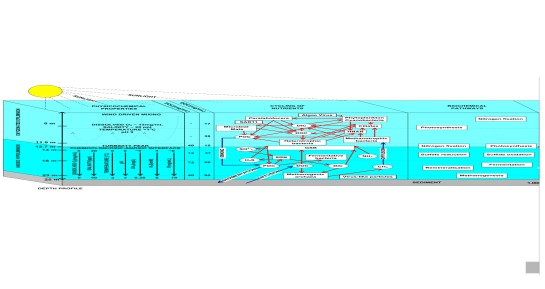
\includegraphics[width=\textwidth]{ace_figures/ace_diagram.pdf}
\caption[Physico-chemical and biological structure of Ace Lake]{Physico-chemical and biological structure of Ace Lake.
In the panel describing nutrient cycling biotic (red arrows) and abiotic (blue arrows) are shown.
The panel describing biochemical pathways shows the labels of the pathways at the depths where they are most significant.
The figure is adapted from \citet{Lauro2011}.
}
\label{fig:ace_diagram}

\end{figure}

It is ice-covered for $\sim$11 months of the year and generally thaws in January \cite{Rankin1999}.
Water is marine-derived and a largely neutral water balance has ensured salinity is close to that of seawater.
The lake is physically separated into an aerobic mixolimnion, a steep chemo/oxycline at 12.7 m and an anoxic monimolimnion.
The monimolimnion is sulfidic and methanogenic; both compounds have presumably accumulated through activity from \ac{SRB} and methanogenic archaea respectively \cite{Rankin1999, Lauro2011} \figref{fig:ace_diagram}.
As a physically and chemically well-characterised system of moderate diversity, Ace Lake was chosen as a model ecosystem to implement a whole systems level analysis to piece together ecosystem functioning.
Samples were obtained from the mixolimnion (5 and 11.5 m), the chemo/oxycline (12.7 m) and the monimolimnion (14, 18 and 23 m ).
Sampling was conducted according the design of the \ac{GOS} expedition \cite{Rusch2007} by using size fractionation of microbial biomass onto 3.0, 0.8 and 0.1 \textmu{}m membrane filters.
Both metagenomic and metaproteomic analysis was conducted on these samples to assess the taxonomic composition, the metabolic potential and identify the active members of the community.

From the metagenomic analysis significant differences were found in taxonomic composition between each size fraction and between the three zones of Ace Lake \cite{Lauro2011}.
The mixolimnion community is similar to a marine surface water assemblage consisting of a high abundance of the SAR11 clade of \emph{Alphaproteobacteria} related to ``\emph{Candidatus} Pelagibacter ubique'' and green algae of the order \emph{Mamiellales}.
However, diversity is reduced by one order of magnitude \cite{Lauro2011}.
Unlike Southern Ocean surface water, the mixolimnion is overrepresented in \emph{Cyanobacteria} related to \emph{Synechococcus} and \emph{Actinobacteria}, which may represent taxa that mark the transition from a marine to lake community.
A dense, near-clonal population of \acl{GSB} related to \emph{Chlorobium} termed \emph{C}-ace reside at the chemo/oxycline at 12.7 m \cite{Ng2010a, Lauro2011}.
Below, in the monimolimnion is a highly diverse community that includes \ac{SRB} and methanogenic \emph{Archaea}.
The viral community comprises \emph{Phycodnaviridae}, \emph{Myoviridae}, \emph{Siphoviridae}, \emph{Podoviridae} and unidentified viral families \cite{Lauro2011}. 
Bacteriophage sequences were abundant in the bottom waters, whereas the surface community, was dominated by phycodnaviruses \cite{Lauro2011}. 

Preliminary metaproteomic analysis along the vertical profile of Ace Lake has been performed using a cross species genomic database comprising the \ac{NCBI} \ac{NR} \cite{Ng2010b}.
A focused metaproteogeonomic analysis conducted on the dense \ac{GSB} layer using the matched \ac{GSB} metagenome as the database resulted in 3-fold increase in protein identifications compared to using the \ac{NR} database \cite{Ng2010b}.
%Put in a table of the rates of matches...
This indicates large gains in metaproteome coverage are possible using a matched metagenomic database \cite{Ng2010b}.
Significantly, \ac{GSB} appeared to be crucial in the lake ecosystem as they had the greatest genetic potential for nitrogen and carbon fixation as well as sulphur cycling \cite{Ng2010b, Lauro2011}.
Metaproteomic analysis was able to identify which proteins were actively expressed and thus the active pathways of the \ac{GSB} metabolism which are crucial to the function of the lake \cite{Ng2010a}.

This study aimed to develop and apply methodologies which provide independant data to complement an integrative metagenomic analysis of the whole Ace Lake ecosystem.
These included a modified epifluorescence microscopy procedure to determine cellular and viral densities and validate the efficacy of size-fractionation and a metaproteomic analysis workflow to identify proteins and estimate their abundance.

%---------------------------------------------------------------------------------------------

\section{Materials and methods}
\label{sec:ace_mm}
\subsection{Ace Lake samples}
Water samples were collected from Ace Lake (68$^{\circ}$28$'$23.2$''$S, 78$^{\circ}$11$'$20.8$''$E), Vestfold Hills, Antarctica on 21 and 22 December 2006. 
A hole positioned above the deepest point (25 m depth) of the lake was drilled through the 2 m ice cover of Ace Lake to reach the lake surface.
A volume of 1--10 L was collected by sequential size fractionation through a 20 \textmu{}m pre-filter directly onto 3.0, 0.8 and 0.1 \textmu{}m pore-size 293 mm polyethersulfone membrane filters \cite{Rusch2007}, along the depth profile.
Two independent sets of filters were obtained, one set for metagenomics and one for metaproteomics.
Filters were placed into sterile 50 ml tubes containing a solution of 2.5 mM EGTA, 2.5 mM EDTA, 0.1 mM Tris-EDTA (pH 8), 1mM PMSF (freshly prepared), 50 \textmu{}l protease inhibitor cocktail VI (Calbiochem, San Diego, \textsc{CA}, \textsc{USA}) and the tubes placed in liquid nitrogen before storage at $-$80$^{\circ}$C.
The protease inhibitor cocktail has a broad specificity for inhibition of serine, cysteine, aspartic and metalloproteases within protein extracts.
Samples were taken in the order, 23, 18, 14, 12.7, 5 and finally, 11.5 m.

After samples from each depth were collected, the sample racks were sequentially washed with 2 $\times$ 25 L 0.1 N NaOH, 2 $\times$ 25 L 0.053\% NaOCl, and 2 $\times$ 25 L fresh water. 
The sample hose was flushed with water from each depth before being applied to the filters. 
A \emph{Chlorobium} signature was identified at 5 m, but not immediately above the \ac{GSB} layer at 11.5 m. 
As the next sample taken after sampling at 12.7 m was at 5 m, and then 11.5 m, despite all equipment being thoroughly washed with bleach, NaOH and water, 
the simplest explanation for the \ac{GSB} signature at 5 m is carry-over from sampling of the dense biomass at 12.7 m. 

A sonde probe (\textsc{YSI} model 6600, \textsc{YSI} Inc., Yellow Springs, \textsc{OH}, \textsc{USA}) was used to record depth, dissolved oxygen content, pH, salinity, temperature and turbidity throughout the water column of the lake. 
Total organic carbon was determined using a total organic carbon analyzer, TOC-5000A (Shimadzu, Kyoto, Japan) equipped with a \textsc{ASI}-5000A auto sampler (Shimadzu), and particulate organic carbon by standard protocols 
\url{(http://www.epa.gov/glnpo/lmmb/methods/about.html)} 
at the Centre for Water and Waste Technology, \textsc{UNSW}.

\subsection{\textsc{DNA} extraction, sequencing and data cleanup}
\textsc{DNA} extraction and Sanger sequencing was performed on 3730xl capillary sequencers (Applied Biosystems, Carlsbad, \textsc{CA}, \textsc{USA}) and pyrosequencing on \textsc{GS20 FLX} Titanium (Roche, Branford, \textsc{CT}, \textsc{USA}) at the \acl{JCVI} in Rockville, \textsc{MD}, \textsc{USA} \cite{Rusch2007}. 
The scaffolds and annotations will be available via \ac{CAMERA} and public sequence repositories such as the \ac{NCBI} and the reads will be available via the \ac{NCBI} Trace Archive. 

Sanger reads were trimmed according to quality clear ranges.
The quality of pyrosequencing reads was assessed as follows: 
a \ac{BLAST} nucleotide database was created from the Sanger reads of the 0.1 \textmu{}m fraction of samples GS230, GS231 and GS232 (see \tabreft{tab:ace_metag} for summary of the metagenomic data and sample IDs).
\input{ace_figures/ace_metag.tex}
After performing a \ac{BLAST} comparison of the corresponding pyrosequencing reads against each Sanger sequence database with a minimum bitscore of 80 and maximum e-value of 0.1, reads were binned according to length.
The percentage of reads for each bin lacking a match to the Sanger read database was recorded. 
The percentage reads at least 25\% repetitive after \textsc{MDUST} \cite{Morgulis2006} analysis at default settings, and the percentage of reads containing N's, were assessed. 
In contrast to earlier pyrosequencers \cite{Huse2007}, no length-dependent bias in reads containing N's was observed. 
However, short reads had a disproportionately high number of repeats. 
Moreover, based on the proportion of reads with no match to the Sanger data set, both very short and very long reads had a disproportionately high number of errors; an observation that was previously reported \cite{Huse2007}.

On the basis of this analysis, a three step filtering process was applied to each sample. 
Reads were initially run through the Celera \textsc{sffToCA} \cite{Miller2008} pre-processor followed by \textsc{Lucy} \cite{Chou2001} and finally, excluding the bottom 8\% and top 3\% of reads determined from the read length distribution. 
As the \textsc{sffToCA} (v5.3) pre-processor removes all reads with a perfect prefix of any other read it overcomes the `perfect duplicates' problem \cite{Gomez-Alvarez2009}.
 
After this process, $<$5\% of the reads belonged to clusters of duplicates with three or more reads, and \ac{COG} of proteins classification of these reads showed an over-representation of category L (replication, recombination and repair) that includes mobile genetic elements, which are often duplicated, suggesting a potential biological significance for the duplicated reads. 
It is possible these residual duplications are a result of high gene copy number or localized fragility of DNA sequences that might be biasing the shear points.

\subsection{Metagenomic DNA assembly and annotation}
Mosaic assemblies were generated for each sample fraction using Celera \ac{WGS} Assembler v5.3 \cite{Myers2000}. 
For each assembly, the runtime parameters used were as outlined for 454 sequencing data in the published standard operating procedure\\ 
\url{(http://sourceforge.net/apps/mediawiki/wgs-assembler/index.php?title 1⁄4SFF\_SOP)}. 
As none of the samples can be considered clonal, these are regarded as stringent assemblies \cite{Rusch2007}. 
Each 0.1 \textmu{}m fraction assembly was a hybrid of Sanger and 454 read data, wherein the estimated genome size was manually set to minimize the number of unitigs from abundant organisms being falsely classified as degenerate \cite{Rusch2007}. 
Annotation of each sample fraction assembly was carried out using an in-house pipeline, wherein the pipeline stages consisted of genomic feature detection and subsequent annotation \cite{DeMaere2011}. 
Detected features consisted of \acp{ORF}, transfer \textsc{RNA} and \ac{rRNA}. 
Each detected \ac{ORF} was further annotated by \ac{BLAST} comparison against \ac{NR}, Swissprot and \ac{KEGG}-peptide sequence databases and by \ac{HMMER} comparison against \ac{TIGRFAM} \cite{Haft2001}, \ac{COG} \cite{Tatusov1997, Tatusov2003} and known marker genes \cite{vonMering2007}.
In all cases the cut-off e-value was a maximum of 1e$-$5. 


\subsection{Epifluorescence microscopy}
Samples of unfiltered lake water and the flow-through from 3.0 and 0.8 \textmu{}m filters from all depths were collected on November 2008 and fixed on site in formalin 1\% (v/v). 
The samples were stored at $-$80$^{\circ}$C for subsequent direct counts of cells and \acp{VLP}. 
Enumeration was performed according to the method of \citet{Patel2007} with modifications. 
Lake water samples were filtered onto 0.01 \textmu{}m pore-size polycarbonate filters (25 mm Poretics, \textsc{GE} Osmonics, Minnetonka, \textsc{MN}, \textsc{USA}). 
Filters were air dried, then placed with the back of the filter on top of a 30 ml aliquot of 0.1\% (w/v) molten low-gelling-point agarose and allowed to dry at 30$^{\circ}$C. 
Samples were stained by the addition of 2 \textmu{}l working solution (1 in 400 dilution in 0.02 \textmu{}m filtered sterile Milli-Q) of \textsc{SYBR} Gold (Molecular Probes, Eugene, \textsc{OR}, \textsc{USA}) to 20 \textmu{}l of mounting medium (\textsc{VECTASHIELD} HardSet, Vector Laboratories, Burlingame, \textsc{CA}, \textsc{USA}). 
Stained samples were counted immediately.
Samples were visualised under wide-blue filter set (excitation 460--495 nm, emission 510--550 nm) with an epifluorescence microscope (Olympus BX61, Hamburg, Germany).


\subsection{Protein extraction}
Proteins were extracted from membrane filters from all 0.1 \textmu{}m fractions from the six depths (5, 11.5, 12.7, 14, 18 and 23 m) according to the protocol developed by \citet{Ng2010a}, which is as follows.
The 0.1 \textmu{}m filters were allowed to thaw at room temperature and cut into quarters asceptically.
Separate extractions were performed on each filter quarter which served as technical replicates.
Each quarter filter was suspended in a lysis buffer containing 10mM Tris-EDTA (pH 8), 20 \textmu{}l of protease inhibitor cocktail VI (Calbiochem), 0.1\% sodium dodecyl sulphate, and 1 mM dithiothreitol.
Three freeze-thaw cycles were performed using liquid nitrogen.
The membrane was then removed, and the buffer was subject to five cycles of sonication of 40 s on a 30 \% duty cycle at power setting of 3, which serves to lyse any remaining cells and shear nucleic acids.
The mixture was centrifuged at 5000 \emph{g} for 25 min at 4$^{\circ}$C to remove insoluble material.
Smaller insoluble particles were removed by filtration through a 0.22 \textmu{}m syringe filter (Millipore, Sydney, NSW, Australia).
Buffer exchange with 30 ml of 10 mM Tris-EDTA (pH 8) and concentration of soluble extracted proteins was performed in a 5 kDa cut-off Amicon Ultra-15 filter unit (Millipore).
Protein concentration was determined using a bicinchoninic acid protein assay kit (Sigma-Aldrich, Sydney, NSW, Australia).

\subsection{Metaproteomic \acs{1D-SDS PAGE} and \acs{LC}-\acs{MS-MS}}
Extracted proteins were separated by \ac{1D-SDS PAGE} containing 12 \% SDS using a Mini-PROTEAN system (Bio-Rad, Sydney, NSW, Australia) as described previously \cite{Saunders2006}.
Trypsin digestion, \ac{LC} and mass spectrometry was conducted according to \citet{Ng2010a} as follows.
The gels were silver stained and the images acquired with a UMAX PowerLook 1000 flat-bed scanner (Fujifilm, Berthold, Vic, Australia).
Each lane containing the size separated proteins were excised and sliced according to size with a sterile scalpel.
Gel slices were washed in sterile Milli-Q water followed by acetonitrile, then subject to a series of reductioin, alkylation and dehydration reactions.
Digestion of proteins with trypsin was conducted by rehydrating gel pieces in a buffer of 200 ng trypsin (Promega, Sydney, NSW, Australia) and 10 mM NH$_4$HCO$_3$ at 37$^{\circ}$C overnight. 
Gel slices were dehydrated in acetonitrile in a centrifugal evaporator (SpeedVac).

Peptides were rehydrated in 1\% formic acid and 0.05\% heptafluorobutyric acid and separated by nano \ac{LC} using an Ultimate 3000 \acs{HPLC} and autosampler system (Dionex, Amsterdam, the Netherlands).
Samples of 2.5 \textmu{}l were concentrated and desalted onto a micro C18 precolumn (500 \textmu{}m $\times$ 2 mm; Michrom Bioresources, Auburn, \textsc{CA}, \textsc{USA}) with H$_2$O:CH$_3$CN (98:2, water to 0.05\% heptafluorobutyric acid) at 20 \textmu{}l min$^{-1}$.
After a 4 min wash, the precolumn was switched into line (Valco 10 port valve; Dionex) with a fritless nano column (75 \textmu{}m $\times$ 10 cm) containing C18 medium (5 \textmu{}, 200 \AA\ Magic, Michrom).
Peptides were eluted using a linear gradient of H$_2$O:CH$_3$CN (98:2, 0.1\% formic acid) to H$_2$O:CH$_3$CN (63:36, 0.1\% formic acid) at 350 nl min$^{-1}$ over 30 min.

1800 V was applied to the low volume tee (Upchurch Scientific, Oak Harbor, \textsc{WA}, \textsc{USA}) and the column tip was positioned $\sim$0.5 cm from the heated capillary (250$^{\circ}$C of an LTQ-FT Ultra mass spectrometer (Thermo Electron, Bremen, Germany).
Positive ions were generated by electrospray and the LTQ-FT Ultra was operated in data-dependent acquisition mode.
A survey scan \emph{m/z} 350--1,750 was acquired in the FT ICR cell (resolution $=$ 1,000,000 ions in the linear ion trap).
Up to the six most abundant ions ($>$3,000 counts) with charge states of $+$2, $+$3 or $+$4 were sequentially isolated and fragmented within the linear ion trap using collision-induced dissociation with an activation $q$ $=$ 0.25 and activation time of 30 ms at a target mass value of 30,000 ions.
\emph{m/z} ratios selected for \ac{MS-MS} were dynamically excluded for 30 s.
Peak lists were generated using \textsc{extract\_msm} from \textsc{Mascot Daemon} (Matrix Science, Thermo, London, \textsc{UK}) using the default parameters.

\subsection{Mass spectra analysis and validation of metaproteomic identifications}
The specta generated from \ac{MS} were searched against the protein sequence database corresponding to that depth constructed from the 0.1 \textmu{}m mosaic assemblies using \textsc{Mascot} version 2.1 (Matrix Science).
\textsc{Mascot Distiller} (Applied Biosystems) was used as the data import filter with the following criteria applied to the \ac{MS-MS} ion search: a maximum of one missed cleavage for trypsin, peptide mass tolerance of $\pm$ 4 ppm, a fragment mass tolerance of $\pm$0.6 Da and variable modifications of acrylamide, carbamidomethyl and oxidation.
The number of protein sequences in each database were as follows: 5 m, 138,208; 11.5 m, 133,948; 12.7 m, 27,142; 14 m, 62,436; 18 m, 71,512; and 23 m, 128,878. 
\textsc{Scaffold} 2.0 (version Scaffold\_2\_05\_01, Proteome Software Inc., Portland, \textsc{OR}, \textsc{USA}) was used to validate \ac{MS-MS}-based peptide and protein identifications. 
Peptide and protein identifications were accepted if they could be established at $>$95\% and 99\% probability, respectively, as specified by the \textsc{Peptide Prophet} algorithm \cite{Keller2002}. 
Protein identifications required the identification of at least two peptides.
 
Proteins that contained similar peptides and could not be differentiated based on \ac{MS-MS} analysis alone were grouped to satisfy the principles of parsimony and are referred to as a protein group. 
Spectral counting was used to semi-quantitively estimate protein abundance. 
The total assigned spectra that matched to each identified protein were exported from \textsc{Scaffold} 2.0. 
For similar proteins that have shared peptides (a protein ambiguity group), spectra were assigned to the protein with the most unique spectra. 
To normalise for variation in total spectra acquired between sample replicates, the number of spectra of each protein was multiplied by the average total spectra divided by the total spectra of the individual replicate. 
The spectral count of each protein was averaged across the replicates. 
As longer proteins are more likely to be detected, the average spectral counts were divided by the length of the protein. 
This value is equivalent to the normalised spectral abundance factor \cite{Florens2006, Zybailov2006}. 
In order to compare the relative abundance of proteins between depths, the normalised spectral abundance factor was divided by the average read depth of the contig (scaffold or degenerate) to which the protein mapped. 

If $>$90\% of a scaffold’s length consisted of surrogate (highly degenerate unitig) sequence, the average read depth of the surrogate was used. 
For identified proteins that were part of a protein group the longest protein length and largest read depth value in the group was used. 
Pairwise comparisons of each zone were conducted on \ac{COG} assigned proteins. 
The normalised spectral counts from each protein was aggregated based on their \ac{COG} annotation. 
All proteins that were part of an ambiguity group were confirmed to share the same \ac{COG} annotation to ensure counts were not biased because of the common spectra.

The summed spectral counts from 5 and 11.5 m (mixolimnion), and 14, 18 and 23 m (monimolimnion) were pooled. 
Statistical significance of differences between each zone was assessed using Fisher's exact test, with confidence intervals at 99\% significance calculated by the Newcombe–Wilson method and Holm-Bonferroni correction (p-value cutoff of 1e$-$5) in \ac{STAMP} \cite{Parks2010}. 
All proteins identified, including their gene identifier, normalised spectral abundance, \ac{COG} and \ac{KEGG} Orthology identifiers, \ac{KEGG} locus tag and matching \ac{COG} or \ac{KEGG} description are provided in the Appendix \tabreft{tab:ace_protids_5m}--\tabreft{tab:ace_protids_23m}.



%---------------------------------------------------------------------------------------------

\section{Results and discussion}

\subsection[Development of an epifluorescence microscopy methodology]{Development of an epifluorescence microscopy methodology}
An epifluorescence microscopy methodology was developed to allow examination of cellular morphology and enumeration of cells and \acp{VLP} in Ace Lake.
Development of a revised method was necessary due to inability to source 25 mm diameter 0.02 \textmu{}m pore-size Anodisc filters (Whatman) that have been long used with fluorescent nucleic acid dyes for this purpose \cite{Hennes1995, Noble1998, Patel2007}. 
They were marked for discontinuation in December 2008 after the take-over of Whatman by \textsc{GE} Healthcare and was the cause of a global shortage that was strongly opposed by the viral ecology community \cite{Torrice2009}.
Since conducting this research, supply of 25 mm Anodisc filters has resumed, albeit at much greater cost per filter. 
The need to develop alternative methodolodies has been great enough that protocols were developed independently by other research groups \cite{Budinoff2011, Diemer2012} stressing the utility of alternatives.

Clear \ac{PCTE} membrane filters were selected for use as a viable alternative product as they have a defined pore-size of sufficiently small diameter (0.01 \textmu{}m) to capture \acp{VLP}. 
Furthermore, they have been used in early studies for \acp{VLP} enumeration \cite{Hara1991, Proctor1992}, have a long history of use with the enumeration of cells \cite{Hobbie1977} and therefore require no new materials to be easily adopted for use.
Finally, use of \ac{PCTE} membranes is approximately 10 times cheaper than the use of Anodiscs and are not subject to drops in availability.
However, \ac{PCTE} membranes have several reported shortcoming that have precluded their standard use for viral enumeration.
The 0.01 \textmu{}m 25 mm \ac{PCTE} filters are difficult to handle compared to 25 mm Anodisc filters that have a plastic support ring around the edge.
Also, \ac{PCTE} filters appear to have higher background fluorescence, have a slow flow-rate taking $\sim$1--1.5 hours to filter 2 ml \cite{Hara1991} and have been reported to give \ac{VLP} counts an order of magnitude lower than that of Anodiscs \cite{Budinoff2011}.%more ref?

The protocol used is detailled in section \ref{sec:ace_mm} \emph{Materials and methods} where the main challenges of using \ac{PCTE} were overcome for the purposes required for this study.
0.01 \textmu{}m pore-size \ac{PCTE} filters can form creases or wrinkles when mounted in the glass vacuum filter.
Good placement of the \ac{PCTE} filter was achieved by touching the edge of the \ac{PCTE} filter against the damp backing filter, making sure it was aligned and then gently and evenly releasing it in a single direction. 
0.01 \textmu{}m pore-size \ac{PCTE} filters also easily become statically charged and will become attracted to surfaces so careful handling is required during manipulation. 
The greatest drawback in the use of \ac{PCTE} filters of such small pore-size is they similarly have a tendency to crinkle when mounted on the glass slide that can make visualisation of cells and \acp{VLP} on a single focal plane difficult.
Agarose was used to embed the filters to help flatten the membrane and aid in mounting.
However, this was not strictly necessary if filters are dried well and pressed flat against the glass slide with a minimal volume of mountant.
Even though careful handling is possible, this method likely requires more technical replicates than Anodisc filters because any \acp{VLP} outside the focal plane will not be counted.
Furthermore, as similarly reported by \citet{Diemer2012} for 0.03 \textmu{}m \ac{PCTE} membranes, distribution of \acp{VLP} on the membrane appears more variable than for Anodiscs with local regions devoid of \acp{VLP} and others with pooling of \acp{VLP}.
The patchier \acp{VLP} distribution was attributed to greater irregularity in pore distribution compared to that of Anodisc filters and was considered to be the main contributing factor to variability in \ac{VLP} counts \cite{Diemer2012}

Back ground fluorescence was at an acceptable level when the SYBR Gold stain is only incorporated into the mountant after filtration rather than staining in the column.
This is one key difference between this protocol and others that use \ac{PCTE} membranes \cite{Hara1991, Proctor1992, Diemer2012}.
Other protocols have used 0.08 \textmu{}m membranes pre-stained with Irgalan Black \cite{Proctor1992} or 0.03 \textmu{}m pre-stained with Sudan black B \cite{Diemer2012} to minimise background fluorescence.
Pre-staining of 0.01 \textmu{}m membranes would be an option for future optimisation of this protocol.

Only one prior report of filtration of natural water onto the \ac{PCTE} membranes with 0.01 \textmu{}m pore-size was found \cite{Hara1991}.
Such a small pore-size necessitates a very strong seal of the filter column against the glass base with no air leaks.
Leakage can be eliminated by sealing the fritted base to the column with laboratory film. 
However, the slow flow-rate was not a property of these \ac{PCTE} filters that could be overcome.
As the filtration and visualisation was performed on fixed samples in the laboratory rather than in the field, the time taken for filtration of 2--3 hours for each sample was not deemed problematic for the purposes of this study.
Counts of \acp{VLP} have been shown to decrease dramatically with time even when preserved with aldehyde-based fixatives \cite{Wen2004}.
Collecting larger sample volumes and flash freezing in liquid nitrogen and storing at $-$80$^{\circ}$C helps to slow this effect \cite{Patel2007}.
Due to logistic contraints of working in the Antarctic, counts in the field were not possible so \ac{VLP} counts are expected to be underestimated.
However, all samples were processed within a similar time frame so the relative \ac{VLP} abundances down the depth profile and between size fractions are expected to be accurate as all samples would have undergone comparable amounts of \ac{VLP} loss. 

Overall, a viable alternative methodology was successfully developed for visualisation and enumeration of cells and \acp{VLP} using \ac{PCTE} membrane filters for use in this study \figref{fig:ace_microscopy}.
\begin{figure}
\includegraphics[width=\textwidth]{ace_figures/ace_microscopy.jpg}
\caption[Epifluorescence microscopy of Ace Lake microbiota]{Epifluorescence microscopy images of Ace Lake microbiota. Scale bar $=$ 20 \textmu{} m. ND, not determined.
}
\label{fig:ace_microscopy}

\end{figure}

To be a competitive alternative to Anodisc filters in terms of enumeration accuracy, further work is required that compares counts using this methodolody and the current standard Anodisc-based protocol \cite{Patel2007} with viral samples of known densities.

%------------------------------------------------------------------------------------------------------------------------

\subsection[Community stratification supported by cell and \acs{VLP} densities]{Size and depth stratification of the community supported by cell and \acs{VLP} densities}

Epifluorescence microscopy images of Ace Lake microbiota showed a clear decrease in larger and particularly filamentous cells between filter size fractions \figref{fig:ace_microscopy}.
The sequential filtration of suspended microbial biomass from aquatic environments has been utilised as part of the landmark Sargasso Sea metagenomic study \cite{Venter2004} and \ac{GOS} expedition \cite{Rusch2007}.
The Ace Lake samples were collected using the same sampling strategy as the \ac{GOS} dataset but has sequence information from all three filter sizes and was able determine if size fractionation is effective at separating the microbial community and if functional differences are associated with size.
Both taxonomic and functional gene composition were shown in the metagenomic analysis to differ significantly with size fraction, particularly between the 0.1 \textmu{}m and the larger size fractions, indicating resource partitioning in the community \cite{Lauro2011}.
The clear difference between the size fractions indicated the sequential filtration process is an effective means to separate the community and that different sized populations in the community have different ecological roles (\emph{e.g.} particle attached copiotrophs or planktonic oligotrophs).
For example, \emph{Flavobacteria} were only detected in the 3.0 \textmu{}m size fraction mixolimnion metagenomes and were inferred to be involved in mineralisation of particulate matter \cite{Lauro2011}.
This correlates with the absence of larger, particularly long rod shaped cells, in the $>$0.8 \textmu{}m microscopic image \figref{fig:ace_microscopy} indicating these larger cells are likely to be copiotrophic \emph{Flavobacteria} involved in degradative processes.
Depth was another variable which strongly drove differences in the Ace Lake community \cite{Lauro2011}.
This was again evident in the microscopy images that show the appearance of long filamentous cells only in the monimolimnion samples \figref{fig:ace_microscopy}.

Cell and \ac{VLP} densities are not obtainable from metagenomic sequence data and necessitates an independent method of determination.
The first studies to determine viral densities in natural systems found that viruses are the most numerous biological entities on the planet and likely play a large role in plankton mortality in the ocean \cite{Bergh1989,Proctor1990}. 
\ac{VLP} counts from marine environments vary with depth and trophic status ranging from 10$^6$ to 10$^8$ \acs{VLP} ml$^{-1}$ \cite{Suttle2005}.
%\ac{VLP} counts from lakes in the Vestfold Hills appear to increase with salinity \cite{Laybourn-Parry2001}.
Both cellular and \ac{VLP} counts are linked with environmental factors such as trophic status \cite{Lauro2009}. 
Enumeration of cells and \acp{VLP} in Ace Lake showed cell densities were lowest in the relatively oligotrophic mixolimnion (0.8--1.3 $\times$ 10$^6$ cell ml$^{-1}$) and were by an order of magnitude higher in the copiotrophic monimolimnion (1.6 $\times$ 10$^7$ cell ml$^{-1}$ in the 23 m sample) \figref{fig:ace_counts}.
\begin{figure}
\centering
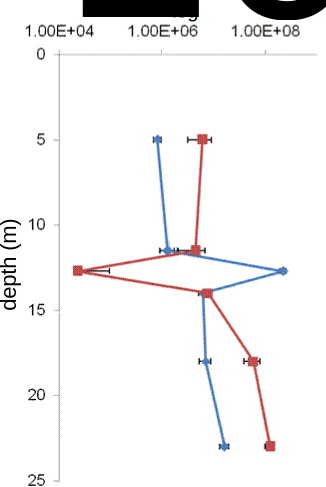
\includegraphics[width=50mm]{ace_figures/ace_counts.pdf}
\caption[Counts of microbial cells and \acs{VLP}s in Ace Lake]{Counts of microbial cells (blue) and \acs{VLP}s (red) by epifluorescence microscopy along a depth profile of Ace Lake.
Error bars represent one standard deviation.
No \acp{VLP} were detected at 12.7 m depth and the value reported represent the detection limit of the counting procedure (\emph{i.e.} one \acs{VLP} detected in one field of view).
}
\label{fig:ace_counts}

\end{figure}

Cell densities were highest at 12.7 m (2.2 $\times$ 10$^8$ cells ml$^{-1}$) corresponding to the \ac{GSB} layer.


\ac{VLP} abundance was consistently higher than the cellular counts but the ratio of \ac{VLP} to cells ranged throughout the water column from $\sim$1--8.5.
The exception to this was the 12.7 m where there was an unusual lack of \acp{VLP} \figref{fig:ace_counts}.
These data corresponded with the metagenomic data from 12.7 m that found no viral signatures associated with the \ac{GSB} at the chemo/oxycline \cite{Lauro2011}.
From metagenomic data alone the absence of viral signatures in the metagenome does not preclude the presence of viruses with ss\textsc{DNA} or \textsc{RNA} genomes that would not be detected by \textsc{DNA} sequencing method used.
Epifluoresence microscopy using SYBR Gold nucleic acid stain would in principle detect \acp{VLP} containing non-dsDNA genomes \cite{Patel2007} that would otherwise be missed in the metagenome.
\figreft{fig:virus_compare} contrasts the epifluorescence images of water from 5 m sample with the 12.7 m sample confirming the lack of visible \acp{VLP} in the latter.
\begin{figure}
\includegraphics[width=\textwidth]{ace_figures/virus_compare.pdf}
\caption[Lack of \acs{VLP} in 5 m and 12.7 m Ace Lake samples]{Epifluorescence microscopy images contrasting Ace Lake water samples from (\textbf{A}) 5 m and (\textbf{B}) 12.7 m. 
Numerous \acp{VLP} are evident in the 5 m sample, but not in the 12.7 m sample. Scale bar $=$ 20 \textmu{}m.
}
\label{fig:virus_compare}

\end{figure}

This provided independent support that the \ac{GSB} population in Ace Lake represents an exception to viral--bacterial population dynamics that describes high rates of genotype cycling in aquatic systems \cite{Rodriguez-Brito2010}.


%---------------------------------------------------------------------------------------------

\subsection[Development of a metaproteomic mass spectra analysis workflow ]{Development of a metaproteomic mass spectra analysis workflow }

Identification of proteins from a microbial community (metaproteomics) indicates which populations or processes are active in the environment and is thus a powerful tool for understanding ecosystems.
However, protein identification by the `shotgun' proteomics approach favoured in metaproteomics \cite{Ram2005} is computationally challenging.
The general shotgun proteomics workflow in \figreft{fig:workflow} shows that apart from successful sample preparation to simplify the complex protein mixture, protein identification depends greatly upon the post-\ac{MS} bioinformatic analysis.
\input{ace_figures/workflow.tex}
This is due to how the \ac{MS-MS} data are used to identify proteins (see \citet{Marcotte2007} for a primer on shotgun proteomic identification).

Briefly, the peptides from digested proteins are separated by \ac{LC} and subject to a round of mass spectra acquisition where the mass of the peptides (precursor ions) are detected.
Selected peptides undergo collision-induced dissociation where they fragment preferentially at the peptide bond.
A second round of mass spectra is acquired of the peptide fragments (fragment ion spectra) that represents the amino acid sequence of the peptide.
An \emph{in silico} enzymatic digestion is performed on a genomic database to predict the precursor ion masses and their corresponding fragment ion spectra.
The fragment ion spectrum and precursor ion mass is used to determine the most likely amino acid sequence of the peptide by comparison to the genomic database and thereby identify the protein(s) of origin.
Since spectral matching depends on extremely high mass sensitivity, the ideal genomic database contains complete coverage of sequences from the organism(s) from which the proteins originated. 
A single amino acid change is sufficient for a peptide match to fail although matching is tolerant to synonymous changes.

Preliminary metaproteomic analysis was conducted on the 0.1 \textmu{}m fraction samples along the depth profile of Ace Lake using sequences from \ac{NR} as the search database \cite{Ng2010b} as metagenomic data were not yet available.
The use of a cross-species database requires the genomes to be sufficiently related to identify proteins and application of stringent statistial cut-off to avoid false-positive matches.
Across all six samples, a total of 10,443 peptides were identified corresponding to 308 proteins from $\sim$400,000 \ac{MS-MS} spectra \cite{Ng2010b}.
Rates of protein identification were low compared to a similar metaproteomic analysis of the Sargasso Sea, which achieved  a total of 5,501 peptide identifications corresponding to 1,042 proteins from $\sim$30,000 \ac{MS-MS} spectra \cite{Sowell2009}. 
This indicated that the Ace Lake community was sufficiently different from relatives in the \ac{NR} database to achieve high rates of protein identification.
A key difference in the Sargasso Sea study was the inclusion of metagenomic sequence in the search database from their target populations of SAR11, \emph{Synechoccocus}, and \emph{Prochlorococcus} \cite{Sowell2009}.
The low identification rate was to be expected as it has been shown that only half the number of proteins are identifiable when using a genomic database that shares 90\% amino acid identity with the matching genome \cite{Denef2007}.

Once the metagenomic sequence for the \ac{GSB} layer became available, re-analysis of the mass spectra to the matched \ac{GSB} metagenome was performed as this sample had the lowest genomic complexity and was expected to obtain high identification rates \cite{Ng2010a, Ng2010b}.
In the re-analysis, 3,970 peptides were identified, mapping to 504 proteins from $\sim$100,000 spectra, which was a near 3-fold increase in the number of protein identifications \cite{Ng2010a, Ng2010b}.
This indicated a similar increase in protein identifications could be achieved with the other Ace Lake samples.
However, metagenomic sequence from more diverse communities adds additional bioinformatic considerations for protein matching due to their inherently greater heterogeneity.
For a protein to be identified according to standard stringency cut-offs it requires at least two peptides to be mapped to it with at least one of those being unique. 
The converse of this is that it allows for the fact there are potentially non-unique peptides shared by other proteins.
Although shared peptides occur between proteins in single genomes, a typical metagenome will contain related species or strains and therefore many more copies of closely related proteins.
%This greatly decreases the probability of finding a unique peptide and thus can exclude proteins from identification.
Protein identification scores in the focussed \ac{GSB} study was also set to only accept identifications above a determined \ac{FDR}.
This is the score given by a peptide match to a randomised version of the genomic database \cite{Ng2010a, Ng2010b}.

To address the additional challenges posed by higher diversity metagenomic data, the program \textsc{Scaffold} 2.0 was adopted for the filtering and validation of peptide and protein matches \figref{fig:workflow}. 
Instead of determining a \ac{FDR}, \textsc{Scaffold} 2.0 employs the \textsc{Peptide Prophet} algorithm \cite{Keller2002} for protein validation.
This algorithm fits a distribution of scores from correct and in-correct peptide matches and from this calculates the probability that each result is a genuine match \cite{Keller2002}. 
More importantly, it identifies groups of proteins that cannot be distinguished based on unique peptides and so accepts all of those proteins in the group may be present in the sample.
Two classes of these groups were defined: (1) protein groups, which are proteins with shared peptides that were indistinguishable from the mass spectral analysis and (2) protein ambiguity groups, which are proteins that have some shared peptides.
This information allows the estimation of protein abundances from spectral counts based on the assumption that proteins that are more abundant will produce more mass spectra.
Spectral counting is only semi-quantitative as differences between low abundance proteins becomes difficult to gauge, and there are likely biases in ionisation and fragmentation efficiencies intrinsic to certain peptides.
For this purpose, defining the protein groups, particularly the ambiguity groups, becomes relevant as it provides a framework to decide how to allocate spectral counts in protein ambiguity groups where spectra are shared.
To find statistically significant differences in protein abundances by spectral counting, several normalisation steps had to be incorporated into the metaproteomic analysis workflow and were implemented using in-house scripts and the statistical program \ac{STAMP}.
This involved normalising the number of spectra between samples, for protein length and for the coverage of the metagenomic sequence and is detailled in section \ref{sec:ace_mm} \emph{Materials and methods}.

The final analysis workflow was applied to all the Ace Lake metaproteomic mass specta datasets.
Appendix \tabreft{tab:ace_protids_5m}, \tabreft{tab:ace_protids_11.5m}, \tabreft{tab:ace_protids_12.7m}, \tabreft{tab:ace_protids_14m}, \tabreft{tab:ace_protids_18m} and \tabreft{tab:ace_protids_23m} lists all proteins identified in Ace Lake using the modified workflow. 
Identification rates were significantly higher using the matched metagenomic database compared to \ac{NR} with a 6-fold increase in total proteins identified \tabref{tab:protid_stats}. 
Mass spectra re-analysed from the 12.7 m \ac{GSB} layer using the modified metaproteomic workflow showed only one additional protein identification \tabref{tab:protid_stats}.
\begin{table}
\footnotesize
\caption[Comparison of proteins identified with \acs{NR} \emph{vs}. metagenomes]{Comparison of the number of peptides/proteins identified in the Ace Lake 0.1 \textmu{}m size fraction metaproteomes using \acs{NR} \emph{vs.} matched metagenomic databases. 
Peptide and protein identifications using \acs{NR} recorded from \citet{Ng2010b}. 
metag, metagenomic database; $a$Proteins identified using \textsc{Scaffold} 2.0; $b$Proteins identified using a \acs{FDR}.}
\label{tab:protid_stats}
\smallskip
\begin{tabularx}{\textwidth}{XXXXXXX}
\toprule
\textbf{Depth (m)} & \textbf{Spectra} & \textbf{Spectra matched (\%) (metag)} &\textbf{Peptide IDs (metg)} & \textbf{Protein IDs (metag)} & \textbf{Peptide IDs (\acs{NR})} & \textbf{Protein IDs (\acs{NR})} \\
\midrule
5     & 71,201  & 10,843 (15) & 5,728  & 501     & 862    & 15 \\
11.5  & 53,078  & 6,076 (11)  & 3,213  & 224     & 327    & 10 \\
12.7  & 127,697 & 29,578 (23) & 12,718 & 505$a$/504$b$ & 4,611  & 169 \\
14    & 100,650 & 9,008 (9)   & 3,427  & 369     & 2,124  & 102 \\
18    & 131,800 & 1,520 (1)   & 725    & 101     & 935    & 11 \\
23    & 232,797 & 3,648 (2)   & 1,602  & 124     & 1,584  & 1 \\
TOTAL & 717,223 & 60,673 (8)  & 27,413 & 1,824   & 10,443 & 308 \\
\bottomrule
\end{tabularx}
\end{table}

This indicates that the \textsc{Scaffold} 2.0 protein validation algorithm is as stringent as \ac{FDR} cut-offs when dealing with lower diversity samples.
In addition, 125 of the 505 protein identifications were identified by \textsc{Scaffold} 2.0 to be protein groups \tabref{tab:ace_protids_12.7m}.
In other words, the mass spectra data were not able to distinguish which of a possible set of two or more proteins were in the sample, or if all the possible proteins that shared those peptides were in the sample.
11 proteins were also found to be part of an ambiguity group and thus shared peptides with other proteins in the sample \tabref{tab:ace_protids_12.7m}.
By tracking protein groups, \textsc{Scaffold} 2.0 flags proteins that require an additional validation step, which is to verify if all members of the group have the same functional annotation.
All protein groups in the 12.7 m sample that were annotated had identical designations indicating they likely had the same function.
The outcomes of the inclusion of spectral counting in the metaproteomic workflow is detailled below.

%---------------------------------------------------------------------------------------------
\subsection[Insights from the metaproteomic analysis of Ace Lake]{Insights from the metaproteomic analysis of Ace Lake}

Metaproteomic identifications were able to support biological inferences about each zone in the Ace Lake community.
Functions defining each zone was indicated at a broad level by overrepresentation of proteins groups assigned to \ac{COG} categories \figref{fig:stamp}. 
\begin{figure}
\centering
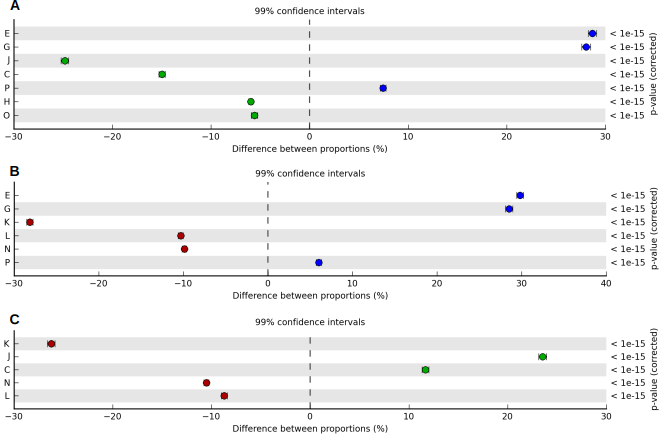
\includegraphics[width=\textwidth]{ace_figures/stamp.pdf}
\caption[Statistical analysis of Ace Lake metaproteome]{ Statistical analysis of normalised mass spectra from \ac{COG} annotated protein between each zone in Ace Lake. 
Proteins are shown grouped into \ac{COG} categories.
Only categories with corrected p-values $<$0.05 and effect size $>$5 are displayed.
(\textbf{A}) Mixolimnion compared to chemo/oxycline. 
(\textbf{B}) Mixolimnion compared to monimolimnion.
(\textbf{C}) Chemo/oxycline compared to monimolimnion. 
Blue, mixolimnion; green, interface; red, monimolimnion.
\ac{COG} category descriptions are: E, amino acid transport and metabolism; G, carbohydrate transport and metabolism; J, translation, ribosomal structure and biogenesis; C, energy production and conservation; P, inorganic ion transport and metabolism; H, co-enzyme transport and metabolism; O, post-translational modification, protein turnover and chaperones; K, transcription; L, replication, recombination and repair; N, cell motility.
}
\label{fig:stamp}

\end{figure}

This gave an indication of how functional processes were separated with depth.
Large numbers of functionally annotated proteins could also be clearly linked to taxonomic groups allowing their contribution to lake ecosystem function and their evolution within the Ace Lake community to be inferred.

\subsubsection{Mixolimnion}
The most abundant proteins in the mixolimnion were assigned to transport functions from COG categories (E) amino acid transport and metabolism, (G) carbohydrate transport and metabolism and (P) inorganic ion transport and metabolism \figref{fig:stamp}. 
Most of the protein identifications could be related to taxonomic groups as well as protein families.
The transporters were predominately \ac{ABC} type, with a high \ac{COG} representation of transporters for carbohydrates ($\sim$34\% of normalised spectra), amino acids ($\sim$32\%) and inorganic ions ($\sim$9\%) (\figreft{fig:stamp}, \tabreft{tab:ace_protids_5m}, \tabreft{tab:ace_protids_11.5m} ).
The prevalence of amino acid and simple sugar transporters and the low \ac{DOC} concentration in the Ace Lake mixolimnion \figref{fig:ace_diagram} is likely to reflect efficient utilisation of these substrates from the \ac{DOC} pool.
Thus, examination of the expressed transport proteins may better indicate substrate preferences and nutritional requirements than measurements of nutrient availability. 

All transporters in the metaproteome were of bacterial origin and conservative phylum level assignments of the normalised spectral abundance showed the majority to originate from \emph{Proteobacteria} (69\%), of which SAR11 comprised 46\% and \emph{Actinobacteria} 19\% (\tabreft{tab:ace_protids_5m}, \tabreft{tab:ace_protids_11.5m}). 
A high proportion of expressed genes with transport functions have also been reported for SAR11 from coastal \cite{Poretsky2010} and open ocean waters \cite{Sowell2009, Morris2010}. 
Oligotrophs, such as SAR11 not only posses a low-diversity of high-affinity transporters \cite{Lauro2009}, but regulate the relative abundance of transporters expressed in response to \ac{DOC} availability \cite{Poretsky2010}. 
The transporter expression profile of the Ace Lake SAR11 was very similar to that of the SAR11 in the Sargasso Sea \cite{Sowell2009}.
Two SAR11 transport proteins that were detected in Ace Lake (\tabreft{tab:ace_protids_5m}, \tabreft{tab:ace_protids_11.5m}) were not detected in the Sargasso Sea \cite{Sowell2009}: an ectoine/hydroxyectoine (167807477 and 167892279) and a zinc \ac{ABC} transporter (167933120). 
Ectoine is a compatible solute and presence of the ectoine transporter indicates it is more availible in Ace Lake than in the ocean, potentially in response to higher variability in salinity or low temperature.
The zinc \ac{ABC} transporter is likely to support zinc efflux in response to zinc concentrations which are $\sim$70-fold higher in the mixolimnion of Ace Lake compared to seawater \cite{Rankin1999}. 
Conversely, phosphate transporters were a major class detected from the Sargasso Sea \cite{Sowell2009} but were absent from the Ace Lake metaproteome consistent with lower phosphate levels in the Sargasso Sea ($<$5 nM) compared to Ace Lake (1--12 \textmu{}M). 
The differences in transporter expression between Ace Lake and oceanic SAR11 are likely to signify adaptive growth strategies that have evolved in the Ace Lake SAR11 community.

\emph{Actinobacteria} sequences were associated with a diverse phylogenetic cluster (Luna cluster) mainly represented by freshwater ultramicrobacteria \cite{Hahn2003}. 
Several Luna cluster isolates contain rhodopsin genes, termed actinorhodopsins \cite{Sharma2009} and similar gene sequences were present in the Ace Lake oxic zone data and found to be expressed (167820670 and 163154474; \tabreft{tab:ace_protids_5m}, \tabreft{tab:ace_protids_11.5m}).
This was the first report of expression of these actinorhodopsin sequences.
The abundance of \emph{Actinobacteria} transporters along with their small cell size and distribution in the water column indicates they occupies a similar ecological niche as SAR11.
SAR11 contains proteorhodopsin which is a related to actinorhodopsin \cite{Sharma2009}.
Although the physiological role of proteorhodopsin in SAR11 is yet to be fully elucidated \cite{Fuhrman2008}, this provides some indication actinorhodopsins in Antarctic Luna cluster \emph{Actinobacteria} have a related functional role.

\subsubsection{Chemo/oxycline}
Proteins from the chemo/oxycline were almost all of \ac{GSB} origin \tabref{tab:ace_protids_12.7m}. 
An in-depth metaproteogenomic analysis of the \ac{GSB} metabolism has been described \cite{Ng2010a, Ng2010b}.
Comparative analysis of proteins between the lake strata showed this depth was more similar to the monimolimnion that the mixolimnion \figref{fig:stamp}.
Compared with the mixolimnion, \ac{COG} categories (J) translation, ribosomal structure and biogenesis; (C) energy production and conservation; (H) co-enzyme transport and metabolism and (O) post-translational modification, protein turnover and chaperones were overrepresented, whereas in comparison with the monimolimnion, only categories J and C were significantly overrepresented.
This difference likely due to the presence of sedimenting \ac{GSB} cells in the monimolimnion.
Nonetheless, overrepresentation of J and C categories indicates it is the \ac{GSB} population at the chemo/oxycline that is the most metabolically active and productive in the whole lake community.
The overrepresentation of category C is similarly evident in the metagenomic comparison of functional genes whereas category J is not \cite{Lauro2011}.
This indicates differences in the regulation of energy metabolism compared to protein translation in \ac{GSB}.

Both metagenomic and microscopic analysis of the \ac{GSB} layer has indicated the population lacks viruses.
Mathematical modeling predicted that the absence of virus predation in the \ac{GSB} could be an adaptation to longer cycles of growth and inactivity in response to the polar light regime \cite{Lauro2011}. 
A mechanism for how virus resistance may be conferred in the population was suggested in the metaproteome.
Abundant \ac{CRISPR} associated \ac{CAS} proteins Cse2, Cse3 and Cse4 (165526330, 165526332 and 165526334, respectively) were detected in the 12.7 m metaproteome \tabref{tab:ace_protids_12.7m}. 
The \ac{CAS} gene locus (cas3, cse1, cse2, cse3, cse4, cas5, cas1b), to which the proteins map, shares its organisation with \ac{CAS} loci of sequenced \ac{GSB}, and groups with the \emph{E. coli} subtype/variant 2. 
The \ac{CRISPR}/\ac{CAS} system has been shown in other organisms to mediate virus resistance \cite{Karginov2010, Horvath2010} and is likely to have a similar function in the Ace Lake \ac{GSB}.


\subsubsection{Monimolimnion}
In parallel with taxonomic diversity increasing with depth, with the exception of the \ac{GSB} layer, the rate of metaproteomic identification of proteins decreased with depth \tabref{tab:protid_stats}.
This is to be expected as complete coverage of all genomic information from an environment is unlikely from all but the most simple of systems which means that as diversity increases there is a greater chance a protein will map to fragmentary or absent metagenomic data and fail to be identified.
Annotated proteins in the monimolimnion were overrepresented in \ac{COG} categories (K) transcription; (L) replication, recombination and repair and (N) motility \figref{fig:stamp}. 
Categories L and N were similarly overrepresented in the monimolimnion metagenomic samples \cite{Lauro2011} demonstrating the genomic expansion of these functions correlated with higher abundance of these proteins.
However, differential adundance was greatest in the category K proteins, which showed showed little difference in relative abundance in the metagenomes \cite{Lauro2011} suggesting transcription proteins in the monimolimnion were up-regulated \figref{fig:stamp}. 
The majority of the proteins that were detected in the monimolimnion (e.g. 67\% at 23 m) \tabref{tab:ace_protids_23m} were for hypothetical proteins that tended to lack orthologues in well-characterized organisms.
This demonstrates the extremely high level of functional novelty in the anaerobic zone of the lake.
These hypothetical proteins represent potential targets for protein expression studies to determine their biological function.


%--------------------------------------------------------------------------------------------
\section{Conclusions}
This study has developed modifications to existing epifluorescence microscopy and metaproteomic methodologies that were successfully applied to the analysis of Ace Lake.
These methods provide independent datasets that complemented metagenomic sequencing.
The epifluorescence microscopy methodology was able to determine the relative difference in cell and \acp{VLP} down the lake profile and may prove to be a viable alternative to Anodisc-based protocols.
Modifications in the bioinformatic analysis of mass spectral data afforded an increase in the number of protein identifications by using the matched metagenome data, identified proteins with shared peptides and enabled estimation of protein abundances by spectral counting.
Both these methodologies have lent crucial bits of data to the integrative understanding of the whole lake ecosystem.
These included validating differences in the microbial community with size and depth, supporting the absence of viruses in the \ac{GSB} layer, trophic status of the lack, describing the transport functions in the lake surface and a potential mechanism for virus resistance in the \ac{GSB}.


%--------------------------------------------------------------------------------------------
\section{Acknowledgements}
This work was supported by the Australian Research Council, the Australian Antarctic Division, the University of New South Wales and the \textsc{NSW} Government. 
The work contributed by members of the \ac{JCVI} was supported by funding from the Gordon and Betty Moore Foundation.
Mass spectrometry and analysis was conducted at the Bioanalytical Mass Spectrometry Facility at the Analytical Centre of \textsc{UNSW}.

\chapter{Virophage Control of Antarctic Algal Host--Virus Dynamics}
\label{ch:olv}

%-----------------------------------------------------------------------------------------------------
\section*{Co-authorship Statement}
\addcontentsline{toc}{section}{Co-authorship Statement}

A version of this chapter has been published as:\\

\textbf{Sheree Yau}, Federico M. Lauro, Matthew Z. DeMaere, Mark V. Brown, Torsten Thomas,
Mark J. Raftery, Cynthia Andrews-Pfannkoch, Matthew Lewis, Jeffery M. Hoffman, John A. Gibson, and
Ricardo Cavicchioli (2011)
Virophage control of antarctic algal host--virus dynamics.\\
\textit{\underline{Proceedings of the National Academy of Sciences USA}}
\textbf{108}: 6163--6168.\\

Contributions to this publication by other researchers is as follows.
Research was designed by Federico Lauro, Mark Brown, Torsten Thomas, John Gibson and Ricardo Cavicchioli.
Sample collection was performed by Federico Lauro, Mark Brown, Torsten Thomas, Jeffery Hoffman and Ricardo Cavicchioli.
DNA extraction and clone library preparation of 2006 samples was performed by Cynthia Andrews-Pfannkoch and Jeffery Hoffman of the J. Craig Venter Institute.
DNA sequencing quality control was performed by Matthew Lewis of the J. Craig Venter Institute.
Metagenomic sequence processing, global assembly and annotation was performed by Matthew DeMaere.
Assistance in mass spectronomy and mass spectra analysis was provided by Mark Raftery.
Assistance in analysis of Eucarya taxonomy was provided by Mark Brown.
Analysis of virophage abundance over time was performed by Federico Lauro.

Apart from these contributions, I performed all other data analyses and interpretations.
\newpage

%----------------------------------------------------------------------------------------------

\section{Abstract}

Viruses are abundant ubiquitous members of microbial communities, and in the marine environment affect population structure and nutrient cycling by infecting and lysing primary producers. 
Antarctic lakes are microbially dominated ecosystems supporting truncated food webs where viruses exert a major influence on the microbial loop. 
Here we report the discovery of a new virophage (relative of the recently described Sputnik virophage) that preys on phycodnaviruses that infect prasinophytes (phototrophic algae). 
By performing metaproteogenomic analysis on samples from Organic Lake, a hypersaline meromictic lake in Antarctica, complete virophage and near-complete phycodnavirus genomes were obtained. 
By introducing the virophage as an additional predator of a predator-prey dynamic model we determine that the virophage stimulates secondary production through the microbial loop by reducing overall mortality of the host and increasing the frequency of blooms during polar summer light periods. 
Virophages remained abundant in the lake two years later, and were represented by populations with a high level of major capsid protein sequence variation (25--100\% identity). 
Virophage signatures were also found in neighbouring Ace Lake (in abundance), and in two tropical lakes (hypersaline and fresh), an estuary, and an ocean upwelling site. 
These findings indicate that virophages regulate host-virus interactions and influence overall carbon flux in Organic Lake, and play previously unrecognised roles in diverse aquatic ecosystems.
\newpage

%---------------------------------------------------------------------------------------------

\section{Introduction}
It has been known for at least 20 years that viruses frequently infect and lyse marine primary producers causing up to 70\% of cyanobacterial mortality \cite{Proctor1990,Suttle1990}.
Eucaryotic phytoplankton are preyed upon by large dsDNA phycodnaviruses (PVs) causing bloom termination in globally distributed species (3,6).
Elevated levels of dissolved organic carbon (DOC) (7) and numbers of heterotrophic bacteria (8-10) occur during algal blooms indicating that viral lysis of eucaryotic algae stimulates secondary production. 
Viruses also suppress host populations at concentrations below bloom-forming levels, with abundance being controlled by the efficiency and production rates of the infecting viruses (11, 12). 

Antarctic lakes are microbially dominated ecosystems supporting few, if any metazoans in the water column (13, 14). 
In these truncated food webs, viruses are expected to play an increased role in the microbial loop (15). 
Low complexity Antarctic lake systems are amenable to whole community based molecular analyses where the role that viruses play in microbial dynamics can be unravelled (14). 
Attesting to this, a metagenomic study of Lake Limnopolar, West Antarctica uncovered a dominance of eucaryotic viruses and ssDNA viruses previously unknown in aquatic systems (16). 

We established a metaproteogenomic program for Organic Lake (68$^{\circ}$27$'$23.4$''$S, 78$^{\circ}$11$'$22.6$''$E), which is located in the Vestfold Hills, East Antarctica, in order to functionally characterize its microbial community. 
Organic Lake is a shallow (7 m) hypersaline ($\approx$230 g L$^{-1}$ maximum salinity) meromictic lake with a high concentration of dimethylsulphide ($\approx$120 $\mu$g $^{-1}$) in its anoxic monimolimnion (17, 18). 
Water temperature at the surface of the lake can vary from $-$14 to $+$15$^{\circ}$C while remaining sub-zero at depth (19, 20). 
The lake is eutrophic, with organic material sourced both from autochthonous production and input from penguins and terrestrial algae. 
The high concentrations of organic material reflect slow breakdown in the highly saline lake water. 
The salt in the lake was trapped along with the marine biota when the lake was formed due to falling sea level c. 3,000 y BP (21, 22). The lake sediment has both low species diversity (Shannon-Weaver diversity: 1.01) and richness (Chao non-parametric index: 32 $\pm$ 12) (23). 
Unlike high latitude lakes, viral abundance has been reported to increase with trophic status (15) and with salinity in Antarctic lakes (24). 

Here we report the analysis of the surface water of Organic Lake, highlighting the presence of a relative of the recently described Sputnik virophage, a small eucaryotic virus that requires a helper \textit{Acanthamoeba polyphaga} mimivirus (APMV) to replicate (25). 
From metagenomic DNA, a complete Organic Lake virophage (OLV) genome was constructed (the second virophage genome to be described), and near-complete genomes of its probable helper Organic Lake phycodnaviruses (OLPVs).

%------------------------------------------------------------------------------------------

\section{Materials and Methods}

\subsection{Samples and DNA Sequencing}
Water samples collected from Organic Lake were: 

\begin{enumerate}
\item Surface water from the eastern side of the ice-free lake (68$^{\circ}$27$'$25.48$''$S, 78$^{\circ}$11$'$28.06$''$E) December 24, 2006.
\item A depth profile collected through a 30 cm hold drilled through the surface ice above the deepest point in the lake (68$^{\circ}$27$'$22.15$''$S, 78$^{\circ}$11$'$23.95$''$E), November 10, 2008. 
\item surface water from the north-east side of the partially ice-covered lake (68$^{\circ}$27$'$21.02$''$S 78$^{\circ}$11$'$42.42$''$E), December 12, 2008. 
\end{enumerate}

Samples were sequentially filtered through a 20 $\mu$m pre-filter and biomass captured onto 3.0, 0.8 and 0.1 $\mu$m membrane filters as described previously (1, 2). 
The samples from 2008 also included 50\% (v/v) RNAlater. 
DNA extraction, sequencing and quality validation was performed as previously described (1, 2). 
DNA sequencing was performed at the J. Craig Venter Institute in Rockville, MD, USA.  

\subsection{Transmission Electron Microscopy}
Unfiltered Organic Lake surface water from December 24, 2006 (fixed on-site in 1\% (v/v) formalin) was concentrated and a solvent exchange performed with sterile filtered ammonium acetate solution 1\% (w/v) using a 50 kDa cut-off Microcon centrifugal filter device (Millipore) according to the manufacturer’s instructions. 
Formvar coated 200 mesh copper grids were floated on a droplet of sample for 30 min, excess liquid wicked off and the grid negatively stained for 30 s with uranyl acetate 2\% (w/v). 
The sample was visualised using a JEOL1400 transmission electron microscope at 100 kV at 150,000 to 250,000 $\times$ magnification.

\subsection{Metagenomic Assembly and Annotation}
Mosaic metagenomic assemblies were generated as previously described (1, 2). 
For the 0.1 $\mu$m Organic Lake 2006 sample, assembly was a hybrid of Sanger and 454 read data (Table S1). 
For all other sample size fractions, runtime parameters used were standard for 454 sequencing data. 
Low GC ($\ge$ 51\%) scaffolds $>$ 10 kb from the 0.1 $\mu$m 2006 assembly had high coverage ($>$ 45 $\times$) indicating these were from the dominant taxa. 
One of these scaffolds was binned as virophage and the rest as PV. 

To further separate the OLPV types and assess the completeness of their genomic content, highly conserved single copy PV orthologues were identified as follows. 
An all against all BLASTp search was conducted with protein sequences from the ten available PV genomes 
(\textit{Acanthocystis turfacea Chlorella} virus 1, PbCV-1, PbCV AR158, PbCV FR483, PbCV NY2A, \textit{Emiliania huxleyi} virus 86, \textit{Ectocarpus siliculosus} virus 1, \textit{Feldmannia} sp. virus, \textit{Ostreococcus} virus 5, \textit{Ostreococcus tauri} virus 1) and APMV (which was included as a close PV relative). 
BLASTp results were parsed and clustered using orthoMCL V1.4 (3, 4). 

Pairs of each orthologue were located on eight of the PV scaffolds. 
The location of each orthologue pair had a complementary distribution so the eight scaffolds were able to be sorted unambiguously into two strains (OLPV-1 and OLPV-2). 
OLPV-1 ribonucleotide reductase $\alpha$-subunit appeared as duplicated on different scaffold ends, likely as an artefact of its proximity to an assembly break point. 
The remaining high coverage scaffolds were searched for predicted proteins present in one OLPV strain but not in the other and assigned to the strain in which it was absent. 
Comparison of OLPV-1 and OLPV-2 scaffolds was performed using tBLASTn of concatenated scaffolds from each strain and visualised using the Artemis Comparison Tool (ACT) (5). 
DNA sequence data is available in Genbank and CAMERA (http://web.camera.calit2.net).

\subsection[Genome Completion and Annotation]{Organic Lake Virophage Genome Completion and Annotation}
The high coverage (77 $\times$), large number of Sputnik homologues that encode essential functions and length of the putative OLV scaffold from the 0.1 $\mu$m 2006 hybrid assembly indicated it was a near-complete genome. 
Reads from this scaffold were reassembled at high stringency and visualised using Phred/Phrap/Consed (6) to complete the sequence. 
Mate-pair data indicated a circular molecule and primers were designed to span the ends of the scaffold and sequence across the gap (Table S5). 
Touch-down PCR was performed with eDNA from 0.1 $\mu$m 2006 sample, the product used for nested PCR and the final product was cloned and sequenced. 
The complete genome was manually annotated and visualised using Artemis (7). 
Translated ORFs (minimal size 120 amino acids) were compared (BLASTp) to GenBank, to the all metagenomic ORF peptide database on CAMERA (http://web.camera.calit2.net) and to predicted proteins from OLPV-1 and OLPV-2 scaffolds. 
Comparisons between the OLV genome and OLPV-1 /OLPV-2 were performed with tBLASTn and visualised using ACT (5). 

\subsection{Phylogenetic Analysis}
Translated amino acid sequences from viral marker genes of interest were retrieved from the 0.1 $\mu$m 2006 metagenomic assemblies from this study, GenBank and CAMERA all metagenomic reads ORF peptide database. Homologous sequences were aligned using MUSCLE v3.6 (8). 
Neighbour-joining analysis, test for clade support (bootstrap analysis 2000 replicates) and tree drawing was performed with Molecular Evolutionary Genetics Analysis (MEGA) software v4 (9). 
Maximum likelihood analysis (JTT substitution model) and test for clade support (aLRT analysis) was performed with PhyML (10) and the tree visualised using MEGA. 
18S rRNA gene sequences were retrieved from reads of all filter sizes, compared (BLASTn, e-value $<$ 1.0e$-$5) to the SILVA100 SSURef database, aligned and phylogeny performed using ARB as previously described (1, 2). 
The abundance and similarity of virophages in all lake samples and filter sizes was estimated using BLASTp (evalue $<$ 1.0e$-$5) to search using the OLV MCP sequence against a database of proteins predicted from sequencing reads. 
The database was generated as previously described (1) and the percent identity of the BLAST hit was used as a proxy for species similarity. 

\subsection{Metaproteomic Analysis}
Metaproteomics of proteins from the 0.1 $\mu$m filter from 2006 was performed as previously described (1, 2), with minor modifications. 
The protein sequence database was generated by combining ORFs from the 3.0, 0.8 and 0.1 $\mu$m mosaic assemblies with 130,581 sequences in the database. 
Scaffold 3.0 (Proteome Software Inc.) was used to validate MS/MS based peptide and protein identifications. 
Protein identification data is available in Table S2. 

\subsection[Algal Host--Virus and Virophage Dynamics]{Model of Algal Host--Virus and Virophage Dynamics}
To model the effect a virophage would have on algal Pyramimonas algal host populations in Organic Lake, modified Lotka-Volterra equations were used describing the OLV as a predator of predator OLPV. 
The original equations are given by:

\begin{equation}
\frac{\mathrm{d}A}{\mathrm{d}t}=\alpha A - \varepsilon PA
\label{eqn:lokprey}
\end{equation}

\begin{equation}
\frac{\mathrm{d}P}{\mathrm{d}t}= \theta PA - \mu P
\label{eqn:lokpred}
\end{equation}

Where:
\begin{description}
\item[$A$] is the number of \textit{Pyramimonas} (prey).
\item[$P$] is the number of OLPV (predator).
\item[$\alpha$] is the specific growth rate of the prey.
\item[$\theta$] is the specific production rate of the predator.
\item[$\varepsilon$] is the rate of predator mediated death of prey.
\item[$\mu$] is the specific decay rate of the predator.
\end{description}

Equation \ref{eqn:lokprey} describes the change in \textit{Pyramimonas} abundance and equation \ref{eqn:lokpred} the change in OLPV abundance in the absence of OLV.
In the presence of OLV, \textit{Pyramimonas}, OLPV and OLV dynamics are described by the following equations:

\begin{equation}
\frac{\mathrm{d}P}{\mathrm{d}t}= \theta PA - \mu P - \omega PV
\label{eqn:pred}
\end{equation}
\begin{equation}
\frac{\mathrm{d}V}{\mathrm{d}t}=\beta PV - \gamma V
\label{eqn:viro}
\end{equation}

Where:
\begin{description}
\item[$V$] is the number of teh OLV (predator of predator).
\item[$\omega$] is the rate of OLV mediated reduction in OLPV infective particles.
\item[$\beta$] is the production rate of OLV.
\item[$\gamma$] is the decay rate of OLV.
\end{description}

Equation \ref{eqn:pred} is a modified version of equation \ref{eqn:lokpred} which includes the effect of OLV on the change in abundance of OLPV.
Equation \ref{eqn:viro} describes the growth properties of OLV as a predator of OLPV.
Values for the variables for the solution shown (Fig. 4) were as follows: initial prey (10), predator (1) and predator of predator (10) numbers, ~$\alpha=$ 0.1, ~$\theta=$ 0.0015, ~$\varepsilon=$ 0.01, ~$\mu=$ 0.01, ~$\omega=$ 0.01, ~$\beta=$ 0.015 and ~$\gamma=$ 0.15. 
COmplex PAthway Simulator (COPASI) software (11) was used to simulate prey, predator and predator of predator dynamics using the deterministic (LSODA) method.
%-----------------------------------------------------------------------------------------


\section{Results and Discussion}
\subsection{Dominance of Phycodnaviruses in Organic Lake}
Water samples from Organic Lake were collected December 2006 and November and December 2008, and microbial biomass collected onto 3.0, 0.8 and 0.1 $\mu$m membrane filters as described previously (14). 
A large proportion of shotgun sequencing reads (96.2\%) from the 0.1 $\mu$m size fraction of the 2006 Organic Lake metagenome (Table S1) had no significant hits to sequences in the RefSeq database 
(tBLASTx with e-value $<$ 1.0e$-$3, minimum alignment length: 60 bp, minimum identity: 60\%). 
The degree of assembly was high, with 77\% of reads forming part of a scaffold, indicating the sample contained a few abundant taxa of minimal diversity. 
Forty-five scaffolds were longer than 10 kb; the five longest ranged from 70 to 171 kb. 
GC content and coverage were used to separate scaffolds into taxonomic groups (Fig. S1). 
A broad division was evident between low ($\le$ 41\%) and high ($\ge$ 51\%) GC scaffolds suggesting they constituted two taxonomic groups. 
All scaffolds in the high GC group that could be assigned contained phage homologues, as did the one exceptional low GC scaffold. 
The low coverage in the high GC group showed bacteriophages were not abundant in the 0.1 $\mu$m fraction. 
These scaffolds were not analyzed further. 
The low GC scaffolds with confident assignments contained sequences matching conserved PV or APMV proteins. 
These PV-related scaffolds comprised 60\% of assembled reads demonstrating that OLPVs were numerically dominant in the 0.1 $\mu$m fraction. 
Transmission electron microscopy (TEM) revealed the presence of virus-like particles with the dimensions and structure typical of PVs (Fig. 1A).

Within the low GC group, scaffolds separated into a high coverage ($>$ 45$\times$) group, including the five longest scaffolds, and a low coverage ($<$ 22$\times$) group. 
Two of the scaffolds in the high coverage group and one in the low coverage group contained the PV marker DNA polymerase B (DPOB). 
The two high coverage DPOB share 76\% amino acid identity and both share ~$\approx$57\% identity to the low coverage DPOB. 
DPOB is single-copy throughout the nucleo-cytoplasmic large DNA virus (NCLDV) family to which PVs belong (26,27), 
demonstrating that the Organic Lake surface waters contained two closely related abundant PV types (DPOB1) and (DPOB2), and a more distantly related lower abundance type (DPOB3). 

Phylogenetic analysis clustered Organic Lake DPOB with unclassified lytic marine PV isolates that infect the prymnesiophytes \textit{Chrysochromulina ericina} (CeV1) and \textit{Phaeocystis pouchetii} (PpV),
 the prasinophyte \textit{Pyramimonas orientalis} (PoV) (4,28), and uncultured marine PVs related to APMV (29, 30) (Fig. 2A and Fig. S2). 
As the host range of PVs broadly correlates with DPOB phylogeny (31, 32), OLPV would infect prasinophytes or prymnesiophytes. 
The most probable host is the prasinophyte, \textit{Pyramimonas} (no prymnesiophyte 18S rRNA gene sequences were present in any size fraction of the Organic Lake metagenome) (Fig. S3).

Supporting the presence of more than one PV, pairs of single-copy PV orthologues 
(ribonucleotide reductase alpha and beta subunits, VV A32R virion packaging helicase, PBCV1 A482R-like putative transcription factor, VV D5 ATPase and VLTF2 family transcription factor) 
were identified in the high coverage scaffolds that shared an average of 81\% percent amino acid identity.
 Based on the positions of single copy genes on the scaffolds and the percent identity between them, the high coverage scaffolds were grouped into two strains designated OLPV-1 and OLPV-2 according to their DPOB phylogeny (Fig. 2A and Fig. S2).
 The remaining high coverage scaffolds were assigned to either strain, resulting in two near-complete genomes of $\approx$300 kb each (Fig. 2C), 
that are within the range of other sequenced PV genomes (155-407 kb). 
In addition, several OLPV genomic fragments contained PV homologues in high coverage scaffolds that could not be confidently assigned to either strain. 

Both OLPV strains contain a PpV-like major capsid protein (MCP) designated MCP1 and another unique MCP designated MCP2 (Fig. 2B and Fig. S4). 
Both OLPV MCP1s were identified in the metaproteome (Fig. 2C and Table S2) but MCP2 was not. 
In addition to MCPs, the metaproteome contained a range of abundant structural proteins and others more likely to be packaged in the virion (e.g. chaperone), that were expressed by OLPV-1, OLPV-2 and/or an OLPV genomic fragment (Fig. 2C and Table S2). 
These data suggest that MCP1 is the major structural protein, and that both OLPV-1 and OLPV-2 were in a productive cycle in the lake at the time of sampling. 

\subsection{Complete Genome of an Organic Lake Virophage}
Sputnik is a small (50 nm) icosahedral satellite virus of mamavirus (a new strain of APMV). 
It was termed a ``virophage'' because co-infection with Sputnik is deleterious to the mamavirus, resulting in abnormal virions and a decrease in mamavirus infectivity (25). 
One 28 kb scaffold in the low GC high coverage group had six out of 38 predicted proteins homologous to Sputnik virophage proteins (Fig. 3 and Table S3), and one PV homologue. 
The scaffold had a low GC content (~$\approx$30\%), similar to the Sputnik genome, and was larger in size (28 kb vs 18 kb for Sputnik). 
Using PCR and sequencing, the scaffold was found to represent a complete circular virophage genome (the Sputnik genome is also circular). Virus-like particles resembling Sputnik in size and morphology were identified by TEM (Fig. 1B).

Sputnik homologues present in the Organic Lake scaffold included the V20 MCP, V3 DNA packaging ATPase, V13 putative DNA polymerase/primase and others of unknown function (V9, V18, V21 and V32) (Fig. 3 and Table S3). 
The Organic Lake virophage (OLV) is distinct to Sputnik as proteins share 27-42\% amino acid identity (28\% MCP identity). 
OLV proteins include OLV9, the homologue of Sputnik V20 MCP, and OLV8, a fusion of the uncharacterised V18 and minor virion protein V19 from Sputnik (Fig. 3 and Table S3). 
The large number of homologues, including genes that fulfill essential functions in Sputnik (V20, V3 and V13), indicate that OLV and Sputnik have physiological similarities. 

\subsection{Gene Exchange Between Virophage and Phycodnaviruses}

As PVs are related to APMV (27) and are abundant in Organic Lake, it stands to reason that OLPV is the helper of OLV. 
In the OLV genome, OLV12 is a \textit{Chlorella} virus-derived gene, indicating that gene exchange has occurred between OLV and PVs (the function of OLV12 is discussed below). 
Similar observations were made for Sputnik, which carries four genes (V6, V7, V12 and V13) in common with the mamavirus, indicative of gene exchange between the viruses and possible co-evolution (25). 
As the V6, V7, V12 and V13 proteins have been associated with virophage-helper specificity, we reasoned that the functional analogues in OLV would have highest identity to proteins from its helper virus, rather than Sputnik. 

By comparing OLV and OLPV, a 7,408 bp region was identified in OLV encoding five proteins (OLV17-22) with identity (32--65\%) to sequences in both OLPV-1 and OLPV-2 (Fig. 2C, Fig. S5 and Table S3). 
OLV20 and OLV13 are collagen triple-helix-repeat-containing proteins, analogous to Sputnik collagen-like proteins (V6 and V7) involved in protein-protein interactions in the APMV virus factory. 
Sputnik can replicate with either mamavirus or APMV as a helper, although coinfection rates are higher with the mamavirus. 
V6 is the only protein with higher identity (69\%) to mamavirus than APMV (42\%) (25). 
Since OLV20 has equivalent identity (63\%) with OLPV-1 and OLPV-2, it appears that OLV may be capable of interacting with both OLPV strains. 
Also within the conserved region, OLV22, is a 141 aa protein of unknown function that only matches sequences from OLPV and the Global Ocean Sampling (GOS) expedition (Table S3). 
Similar to OLV22, Sputnik V12 is a small protein (152 aa) of unknown function with high identity to APMV, and both may mediate a specific helper-virophage interaction. 
Other genes in this region of OLV can be mapped to OLVP, including a putative transmembrane protein (OLV17) and paralogous phage tail fibre repeat containing proteins, OLV18 and OLV19. 
Analogous to the collagen-like proteins, OLV19 and OLV20 probably facilitate interactions between helper and virophage. 

OLV12 (which is unique to OLV) consists of a C-terminal domain present in conserved hypothetical \textit{Chlorella} virus proteins and an N-terminal domain most closely related to class 3 lipases that may confer OLV selectivity to a PV. 
OLV12 may function similarly to the Sputnik V15 membrane protein in modifying the APMV membrane (25). 
The Sputnik V13 consists of a primase domain and SF3 helicase domain related to NCLDV homologues, involved in DNA replication. 
The helicase domain of OLV25 and V13 are similar, although the primase domain is more similar to a protein from \textit{Ostreococcus lucimarinus}, implying a past association of OLV with a prasinophyte alga host. 

Genes unique to OLV point to adaptations specific to its helper-host system. 
Most notably, OLV possesses a N6 adenine-specific DNA methyltransferase, as does OLPV. 
In OLPV-1, genes for a bacterial type I restriction modification (RM) system are adjacent to a gene encoding a type I methylase-S target recognition domain protein, and upstream of a DNA helicase distantly related to type III restriction endonuclease (RE) subunits. 
A large number of \textit{Chlorella} virus genomes have both 5mC and 6mA methylation (33), and several contain functional RM systems (34). 
The prototype \textit{Chlorella} virus PbCV-1 possesses REs packaged in the virion for degrading host DNA soon after infection (35). 
In contrast to OLV/OLPV, DNA methyltransferases are absent in both Sputnik and APMV, indicating that the N6 adenine-specific DNA methyltransferase has been selected in OLV to reduce endonucleolytic attack mediated by OLPV. 

\subsection[Virophage in Algal Host--Phycodnavirus Dynamics]{Role of Virophage in Algal Host--Phycodnavirus Dynamics}
The presence of the virophage adds an additional consideration to the microbial loop dynamics. 
In batch amoeba cultures, co-infection of amoeba with APMV and Sputnik causes a 70\% decrease in infective AMPV particles and a 3-fold decrease in lysis (25). 
To test how OLV affects OLPV and host population dynamics, we modelled the OLV as an additional predator of a predator in a Lotka-Volterra simulation (Fig. 4). 
In the model, the effect of virophage is robust, with equilibrium solutions across a wide range of parameter values (Fig. 4 shows one equilibrium solution). 
By decreasing the number of infective OLPVs, the presence of OLV shortens the recovery time of the host population (Fig. 4C) and shifts the orbit away from the axis (Fig. 4D). 
The model reveals that the virophage stimulates the flux of secondary production through the microbial loop by reducing overall mortality of the host algal cell following a bloom, and by increasing the frequency of blooms during the summer light periods. 
Antarctic lake systems have evolved mechanisms to cope with long light-dark cycles (14) and shortened trophic chains. 
In Organic Lake and similar systems, a decrease in PV virulence may be instrumental in maintaining stability of the microbial food web. 

\subsection{Ecological Relevance of Virophages in Aquatic Systems}
Metagenomic analysis of Organic Lake samples taken two years later in November (when the lake was ice covered) and December 2008 (partially ice-free) revealed sequences with 99\% amino acid identity to OLV MCP indicating persistence of OLV in the ecosystem (Fig. 5 and Table S4). 
In addition, sequences with lower identity (25--90\%) were detected, particularly in December, demonstrating Organic Lake virophages are highly diverse but OLV remained the dominant type. 

From surface water samples of nearby Ace Lake (meromictic, surface 2\% salinity), a large number of sequences were obtained that matched both the OLV MCP (Fig. 5 and Table S4) and PVs (14). 
All Ace Lake size fractions contained matches to OLV MCP, some with high identity (80--100\%) and the majority with greater variation (25--80\% identity) (Fig. 5 and Table S4). 
In contrast to Organic Lake where the largest number of matches was to the 0.1 $\mu$m size fraction, the majority of Ace Lake sequences were from the larger fractions (Fig. 5 and Table S4). 
This indicates the Ace Lake virophages were associated with host cells during sampling, or possibly with helper viruses that are larger than the OLPVs. 

Extending the OLV MCP search to the GOS data revealed matches (25-28\% identity) to sequences from the hypersaline Punta Cormorant Lagoon (Floreana Island, Galapagos), an oceanic upwelling near Fernandina Island (Galapagos), Delaware Bay estuary (NJ, USA), and freshwater Lake Gatun (Panama) (Table S4). The phylogenetic analysis of a conserved 103 amino acid region of the MCPs revealed a number of clusters, with Sputnik clustering with virophage sequences from Ace Lake that had low identity (22\%) to OLV MCP (Fig. 5 and Fig. S4). 
To improve searches for virophages and better understand their physiology and evolution, it will be valuable to target more genomes (e.g. the Ace Lake 167858124 relative with 40\% MCP identity to Sputnik) and determine which genes are core to virophages and what relationship exists between genome complement and MCP identity.
 
In view of the implications of the virophage modelling (Fig. 4), the abundance and persistence of OLV in Organic Lake (Fig. 5, Table S4), and the presence of diverse virophage signatures in a variety of lake systems (fresh to hypersaline), an estuary, an ocean upwelling site and a water cooling tower (Sputnik), our study indicates that numerous types of virophages exist and play a previously unrecognised role in regulating host--virus interactions and influencing ecosystem function in aquatic environments. 

%------------------------------------------------------------------------------------------------------

\section{Acknowledgements}
We thank Craig Venter, John Bowman, Louise (Cromer) Newman, Anthony Hull, John Rich and Martin Riddle for providing helpful discussion and logistical support associated with the Antarctic expedition, and Lisa Ziegler for discussion about marine viruses. 
We acknowledge technical support for computing infrastructure and software development from Intersect, and in particular assistance from Joachim Mai. 
This work was supported by the Australian Research Council and the Australian Antarctic Division. 
Funding for sequencing was provided by the Gordon and Betty Moore Foundation to the J. Craig Venter Institute. 
Mass spectrometric results were obtained at the Bioanalytical Mass Spectrometry Facility within the Analytical Centre of the University of New South Wales. 
This work was undertaken using infrastructure provided by NSW Government co-investment in the National Collaborative Research Infrastructure Scheme. 
Subsidized access to this facility is gratefully acknowledged. 
We thank Jenny Norman from the UNSW Electron Microscopy Unit her assistance in generating images. 

\chapter[Organic Lake]{Heterotrophic resourcefulness and unusual sulphur biogeochemistry in a hypersaline Antarctic Lake}
\label{ch:org}
\acresetall

%---------------------------------------------------------------------------------------------
\section*{Co-authorship Statement}
A version of this chapter has been submitted as:\\

\textbf{Sheree Yau}, Timothy J. Williams, Federico M. Lauro,  Matthew Z. DeMaere, Mark V. Brown, John Rich, 
John A.E. Gibson, Ricardo Cavicchioli. 
Heterotrophic resourcefulness and unusual sulfur biogeochemistry in a hypersaline lake.
\emph{\underline{ISME Journal}}
submitted, 2013.

Contributions to this manuscript by other researchers is as follows.
Research was designed by Federico Lauro, Mark Brown, John Gibson and Ricardo Cavicchioli.
Sample collection was performed by Federico Lauro and Ricardo Cavicchioli.
Metagenomic sequence filtering, global assembly and annotation was performed by Matthew DeMaere.
Assistance in analysis of functional gene markers provided by Timothy Williams.

Apart from these contributions, I performed all other data analyses and interpretations.
\newpage

%----------------------------------------------------------------------------------------------

\section{Abstract}
Organic Lake is a shallow, marine-derived hypersaline lake in the Vestfold Hills, Antarctica that has the highest reported concentration of dimethylsulphide \ac{DMS} in a natural body of water.
To determine the composition and functional potential of the microbial community and learn about the unusual sulfur chemistry in Organic Lake, shotgun metagenomics was performed on size fractionated samples collected along a depth profile.
Eucaryal phytoflagellates were the main photosynthetic organisms.
Bacteria were dominated by the globally distributed heterotrophic taxa \emph{Marinobacter}, \emph{Roseovarius} and \emph{Psychroflexus}.
Candidate division RF3 was overrepresented at the oxycline and OD1 in the lake bottom.
The dominance of heterotrophic degradation coupled with low fixation potential indicates possible net carbon loss.
However, abundant marker genes for aerobic anoxygenic phototrophy, sulfur oxidation, rhodopsins and CO oxidation were also linked to the dominant heterotrophic bacteria and may indicate use of photo- and lithoheterotrophy as mechanisms for conserving organic carbon.
Similarly, a high genetic potential for the recycling of nitrogen compounds likely functions to retain fixed nitrogen in the lake.
\ac{DMSP} lyase genes (\emph{dddD}, \emph{dddL} and \emph{dddP}) were abundant indicating \ac{DMSP} is a significant carbon and energy source.
Unlike marine environments, \ac{DMSP} demethylases (\emph{dmdA}) were less abundant than \ac{DMSP} lyases indicating that \ac{DMSP} cleavage is the likely source of the high \ac{DMS} concentration.
Strategies of nutrient resourcefulness such as \ac{DMSP} cleavage, carbon mixotrophy (photoheterotrophy and lithoheterotrophy) and nitrogen remineralization in dominant Organic Lake bacteria are potentially important adaptations to nutrient constraints.
In particular, carbon mixotrophy reduces the extent of carbon oxidation for energy production allowing more carbon to be used for biosynthetic processes.
The study sheds light on how microbial communities and the functional processes they perform evolve in response to unusual environmental conditions.

\newpage

%---------------------------------------------------------------------------------------------
\acresetall
\section{Introduction}
Molecular biology approaches have proven useful for describing the diversity and gene content of microorganisms in Antarctic lakes and for inferring the functional roles of the taxa present \cite{Laybourn-Parry2007}.
However to date, only a few large scale shotgun metagenome studies have been performed on the Antarctic continent and in the surrounding Southern Ocean \cite{Wilkins2012a}. 
In the Vestfold Hills, metagenomics and metaproteomics have been used to study Ace Lake (68$^{\circ}$28$'$23.2$''$S, 78$^{\circ}$11$'$20.8$''$E) and Organic Lake (68$^{\circ}$27$'$23.4$''$S, 78$^{\circ}$11$'$22.6$''$E) \cite{Ng2010a, Lauro2011}.
For Ace Lake, a comprehensive assessment of the community structure, biogeochemical fluxes and responses to resource limitation have been described \cite{Lauro2011}.
The metabolism of abundant green sulphur bacteria \cite{Ng2010a} was found to play a central role in nutrient cycling and a mathematical model was developed that showed its dominance was dependent on synchronicity with the polar light cycle leading to absence of phage predation \cite{Lauro2011}.
For Organic Lake, a member of the virophage virus family was discovered that potentially regulates microbial loop dynamics \cite{Yau2011}. 
The Organic Lake virophage likely depends on phycodnaviruses (algal viruses) and it was predicted that the virophage would reduce infective phycodnaviruses leading to an increased frequency of algal blooms and thus carbon flux \cite{Yau2011}.
Virophage sequences were also identified in a range of aquatic metagenomes revealing that they are likely to play ecologically important roles in many aquatic systems \cite{Yau2011}. 
These studies on Ace and Organic lakes both used shotgun metagenomics and illustrate the value of adopting a metagenomics approach for learning about microbial ecology in Antarctic environments.

Due to the polar light cycle, phototrophic growth in Antarctic environments is relatively high in summer and negligible in winter \cite{Laybourn-Parry2005} and requires microbial life to survive under long periods under a scarcity of resources.
To overcome this limitation, Eucaryotic phytoflagellates in Ace Lake engage in carbon mixotrophy by grazing on bacterioplankton to supplement their carbon requirements in the winter \cite{Laybourn-Parry2005}.
Heterotrophic marine bacteria can be similarly resourceful by exploiting light energy through photoheterotrophic processes including \ac{AAnP} or via use of rhodopsins, or lithoheterotrophy such as oxidation of carbon monoxide \cite{Moran2007b}.

Organic Lake is shallow (6.8 m) and has variable surface water temperatures ($-$14 to $+$15 $^{circ}$C) while remaining sub-zero throughout most of its depth \cite{Franzman1987b, Gibson1991, Roberts1993, Gibson1999}.
The salt and marine biota in the lake originate from seawater that was trapped in a basin ~3 000 y BP \cite{Zwartz1988, Bird1991}. 
The bottom waters of Organic Lake are unusual due to the absence of hydrogen sulphide and the high concentration of the volatile gas \ac{DMS} \cite{Deprez1986, Franzmann,1987b, Gibson1991, Roberts1993a, Roberts1993b}. 
Concentrations of \ac{DMS} as high as 5 000 nM have been recorded in Organic Lake \cite{Gibson1991}, 100 times the maximum concentration recorded from seawater in the adjacent Prydz Bay and at least 1 000 times that of the open Southern Ocean \cite{Curran1998}.
More than forty years ago atmospheric DMS was proposed to have a regulatory effect on global cloud cover as it is a precursor of cloud condensation nuclei (Lovelock and Maggs, 1972; Charlson et al., 1987).

%------------------------------------------------------------------------------------------

\section{Materials and methods}

%-----------------------------------------------------------------------------------------


\section{Results and discussion}

%------------------------------------------------------------------------------------------------------

\section{Acknowledgements}

\chapter{Ace Lake Viral Genomes}
\label{ch:viruses}

\chapter{General discussion, conclusions and future work}
\label{ch:conc}
\acresetall

\section{Summary of the major achievements of this work}

%Development of microscopy and metaproteomics applied to subsequent studies.
%These methods are not perfect but they'll do.
%GSB were able to be described totally without culturing.
Proof of concept of the approach.
Totally new discoveries have made testable hypotheses.

\section{Future work}
\subsection{Ace Lake}
%Dynamics over the whole year.
%What happens to the lake during the winter? 
%Can we isolate them.
%Are they endemic or do they change?
%Can we

\subsection{Virophages}
Since the discovery of the \ac{OLV} \cite{Yau2011} described in chapter \ref{ch:olv}, two other members of the virophage family have been reported.
The first of these is the Mavirus (for Maverick virus) so named for its evolutionary relationship with the Maverick/Politon class of eucaryotic transposons \cite{Fischer2011}.
Like Sputnik, Mavirus appears to have an absolute requirement for a giant `helper' virus of the \ac{NCLDV} group to replicate.
In this case \ac{CroV} is the helper virus, which replicates in the cellular host \emph{Cafeteria roenbergensis}, a marine heterotrophic nanoflagellate. 
Also like Sputnik, addition of Mavirus during \ac{CroV} infection leads severe drops in production of \ac{CroV} \cite{Fischer2011}.
The other virophage reported was called Sputnik 2 (its genome is virtually identical to Sputnik) and like Sputnik was also found in association with strain of mimivirus, named lentille virus \cite{Desnues2012}.
Unlike Sputnik, it was found both as a free virion and integrated in the lentille virus genome \cite{Desnues2012}.

The availability of these new virophages in culture affords a new perspective on \ac{OLV} and virophages in general.
In first place, the inability for Mavirus to infect without \ac{CroV} and its detrimental effect on \ac{CroV} just like Sputnik strengthens the assumption that OLV would similarly have a 'virophage' phenotype \ac{OLPV}.
This is in part because Mavirus and \ac{CroV} and quite divergent from Sputnik and mimivirus respectively, yet retain the same traits \cite{Fischer2010, Fischer2011}, suggesting the 'virophage' phenotype is common to the whole lineage.
Secondly, these cultured virophages offers some mechanistic reasons for why \ac{OLV} would function as the other virophages.
As both mimivirus and \ac{CroV} encode a great deal of their own replication and transcription machinery, including all \textsc{DNA} and \textsc{RNA} polymerase subunits, they do not localise to the nucleus during infection but generate the viral factory in the cytoplasm \cite{LaScola2008, Fischer2011}.
Sputnik and Mavirus replicate exclusively in the giant virus factory and make use of the helper virus replication and transcription systems \cite{LaScola2008, Fischer2011}.
Furthermore, Sputnik and Mavirus share the promoter and other transcriptional control sequences of their helper viruses \cite{Claverie2009, Fischer2011}.
They therefore are primarily parasitising the resources of the helper viruses, which seems a likely cause of reduced helper virus production \cite{Claverie2009, Fischer2012}.
\ac{OLPV}-1 encodes all eight \textsc{RNA} polymerase subunits (see GenBank accession HQ704802) indicating it, like all other members of the mimivirus lineage, would replicate solely in the cytoplasm.
Therefore, it is likely \ac{OLV} would exclusively utilise its helper virus' molecular machinery to similarly detrimental effect.
Ultimately, definitely determining if this is the case for the \ac{OLV} would require isolating it from the environment.

Comparison of three different virophage genomes has raised tantalising questions about virophage physiology, evolution and ecology
All three genomes have share homologues of the Sputnik V20 \ac{MCP}, V3 FstK-HerA DNA packaging ATPase and V9 putative cysteine protease but otherwise are quite divergent.
%Sputnik and Mavirus additionally share a the V13 primase/superfamily 3 helicase and the V14 Zn-ribbon domain containing protein.
%While Sputnik and \ac{OLV} share the V18/19 minor virion protein, V1 primase-polymerase containing protein and V21 hypothetical protein.
Mavirus, in particular, is in many ways more similar to the Maverick/Politon transposable elements in the possession of a retroviral-family integrase that is absent in Sputnik and \ac{OLV} \cite{Fischer2011}.
This was theorised to have been separately acquired as a way to stabilise the relationship between the ancestral Mavirus and its cellular host as integration of a virophage could perhaps serve as a defence against infection of the giant helper virus \cite{Fischer2011}.
In support of this, Mavirus can be independently phagocytosed by \emph{Cafeteria roenbergensis} in the absence of \ac{CroV} -- potentially to reduce the severity of a subsequent \ac{CroV} infection \cite{Fischer2011}.
As yet Mavirus has not as yet been reported to be integrated in the host \emph{Cafeteria roenbergensis}.
In contrast, Sputnik seems to associate directly with the fibrils that coat the mimivirus virion, not the host \emph{Acanthamoeba} cell \cite{Boyer2011}.
These two modes of infection, that is a virophage--host interaction followed by helper \emph{vs}. helper--virophage co-infection of host cell, would lead to distinct effects on the population dynamics in the environment.
Detection of \ac{OLV} genome as a separate circular molecular in the 0.8-- 0.1 \textmu{}m size fraction (Chapter\ref{ch:olv}) indicates it is somehow in association with larger particles.
Determination of the mode of infection for \ac{OLV} would improve predictive modelling of \ac{OLV} driven impacts on algal blooms.
This could be achieved by observation of \ac{OLV}-\ac{OLPV} infections in culture or flow cytometric sorting of sample populations of potential hosts and \ac{OLPV} from the environment and screening of the presence of \ac{OLV}.
The latter experiment would also establish fundmental properties of \ac{OLV} such as the identity of hosts and helper viruses, proportions of infected cells and proportions of \ac{OLPV} infections that include an \ac{OLV}.
 
The discovery that Sputnik 2 can integrate into its helper lentille virus suggests a similar interaction could occur between \ac{OLV} and \ac{OLPV}.
This is because integration of Sputnik 2 is localised to a 352 bp region shared by Sputnik 2 (corresponding to the Sputnik V6 gene), lentille virus and mamavirus  \cite{Desnues2010} that encodes a collagen-like repeat-containing protein.
\ac{OLV} and \ac{OLPV} shared a homologous collagen-like repeat-containing protein (Chapter\ref{ch:olv}) that may similarly function as a site of integration.
As yet, the conditions and mechanism by which Sputnik 2 integrates is unknown.
From the metagenomic sequence, \ac{OLV} assembled as a separate molecule (Chapter\ref{ch:olv}).
Screening of metagenomic assemblies from other sampling dates, such as Ace lake and the 2008 Organic Lake samples, for \ac{PV) genomes with integrated virophages can be performed to see if this occurs in the environment at different times.
Again, obtaining isolates or assembling more \ac{PV} genomes can determine if this is a common trait in other virophage systems.
If integration occurs between \ac{OLV} and \ac{OLPV} it would have interesting implications for their natural dynamics.
One interesting possibility is that integration of virophages may function analogously to lysogeny in bacteriophages if integration lead to a `dormant' state for the virophage.
In this scenario, virophages would then integrate into their helper virus when helper virus densities are low to avoid driving their helpers to extinction.
On the other hand, if integration does not entail dormancy of the virophage, it could function as a means to ensure transmission.

%%%OLV physiology questions
%Need to isolate to determine if detrimental
%Determine which OLPV type it infects.
%Verify OLPV infects pyramimonas.
%Verify OLV reduces infective particles.

%%%OLV dynamics questions
%Make an exclusion experiment to show that the dynamics change with and without the OLV. 
%The single cell screening experiment.
%and track them over a season.

%%%OLV distribution and evolution questions
%virophages seem to attack only mimivirus relatives.
%How common are they in the environment?
%They seem like an ancient lineage, how widespread are they? Do they infect other NCLDV


Need future work on organic lake whole lake
%Need to show that AAnP genes are expressed with RT-PCR, proteomics
%Future experiments can look at fluorescence of bchlA
%Cloning of the dddD, dddL genes into appropriate host to show activity.
%Look for inputs into the lake.
%Is allochtonous inputs feeding the lake?
%Need to show the dynamics of the lake
%Need to look at the rest of viral community 

Perspective of Antarctic Lake research from wetlab to molecular age.

Assessment of the value of molecular antarctic research
%Molecular data can be continued to be mined! 
%Serves as a record for prosterity
%Metagenomics is not enough! There needs to be functional data, single cell data, biochemical data.



%Endmainmatter-------------------------------------------------------------------------------------

%Endmatter-----------------------------------------------------------------------------------------

\singlespacing
\bibliographystyle{mybibstyle}
\bibliography{Thesis}


\chapter{Appendices}
\label{ch:appen}

\begingroup
\footnotesize
\begin{longtable}{p{1.5cm}p{6cm}p{6cm}}
\caption[Peptide data for Organic Lake metaproteomics analysis]{Peptide data for Organic Lake metaproteomic analysis. $a$Proteins that have some shared peptides; $b$162322406 and 162276024 are protein homologues; $c$A group of proteins containing similar peptides that could not be differentiated by the mass spectral analysis. Only one gene number of that groups is displayed.}
\label{tab:peptides}
\\
\toprule
\textbf{Gene ID} & \multicolumn{2}{l}{\textbf{Peptide sequences}} \\
\midrule
\endfirsthead
\multicolumn{3}{c}
{\tablename\ \thetable\ -- \textit{Continued from previous page}} \\
\toprule
\textbf{Gene ID} & \multicolumn{2}{l}{\textbf{Peptide sequences}} \\
\midrule
\endhead
\bottomrule \multicolumn{3}{r} {\textit{Continued on next page}} \\
\endfoot
\bottomrule
\endlastfoot
162322530$a$ & R.AIDECLWAVSSLSPSSSADVK.V & R.LNFNHPCK.E \\
  & K.ALGAQPFNYTDAVDALPNSIK.A &  K.LQLNGQDR.F \\
  & R.EGTYFDQVQPFQHHTR.Y & R.NGDLAYR.T \\
  & R.HSNFAMESIEQTFNGQADFGR.R & R.NYNVLR.I \\
  & K.HYGDWMQIWCQLTLDK.N & R.QVCAPR.N \\
  & R.IDNATLQLVLSNATVEGTNTAK.V & R.RVNCTISR.N \\
  & K.INLDLR.A & R.VNCTISR.N \\
162322348 & K.GNVDVYQENK.L & K.IESDAEPSWVR.G \\
162322406$b$ & R.QNQSCGGVNQVNGTHVNR.T  & K.TNDGTLVGK.S\\
  & R.TAFHLGDGLSR.Q & K.YVSESSTYTR.F \\
162313481 & K.ITTIPENIGQLVK.I & R.SNLQGVTEEQLMSNK.I \\
162276060 & K.TPTGLEFSLTGR.A  & R.VNHTDACSTGNK.E \\
162300260 & R.VDIEGGTPFFLK.E & K.YTFQPSELSNTYFSK.E \\
162276024$b$ & K.LGGGISSR.S & R.TSLHMGDVLSR.K \\
  & R.SEVGFQSTMVGSDVAMQR.K & \\
162275992 & K.NINLLSAGANYGINTVGSSLR.N  & R.NPNLQIR.S \\
162300108 & K.NDNIITLLDTK.Q & K.YENGSWNTLGQLIR.G \\
  & K.NVVINSEGTIISAVNNK.G & R.LTVNNSIISK.E \\
  & K.QDVITDQTNLNVGR.L & \\
162319393$a$ & R.AIDECLWAVNTLSPDSSSDVK.V & K.LQLNGQDR.F \\
  & K.ALGAQPFNYTDAIDALPNSVK.A & R.NGDLAYR.T \\
  & R.EGTYFDQVQPFQHHTR.S & R.NYNVLR.I \\
  & R.IDNATLQLVLSNATVEGTNTAK.V & R.QVCAPR.N \\
  & R.IMSGMGGLAYSN & R.RVNCTISR.N \\
  & K.INLDLR.A  & R.VNCTISR.N \\
  & R.LNFNHPCK.E \\
162300134$c$ & K.ATAGDTHLGGEDFDNR.M & R.VEIIANDQGNR.T \\
  & R.IINEPTAAAIAYGLDK.K & \\
162286324$c$ & K.DVPLVANFSAK.F & K.MKLENTVEK.M \\
OLV9 & K.AGLLSEMDAYSLYQMSR.R & R.NGSQQTWNEFR.G\\
  & K.ELVLSFSSGVK.F & K.NILPYDEFVAYK.T\\
  & K.FGTQASTLFLK.D & F.NVNVPSENTLVDR.N\\
  & R.GSSATMSGLLTK.S & K.SEVLEAK.E \\
  & K.GVASAVESAIGGAK.T & K.VSVQSADILNVITK.Q \\
  & K.HIQTTPSMVDK.Y & R.YISLHPSQYAK.L \\
  & R.ITSDVQVAVK.D  & K.YTSLGSIIVIDPVR.D \\
  & K.IYLVVRPQYR.S & \\
OLV8 & K.AGTPIPGVIYEPSYPR.W & K.TLPVFIPTIK.Y \\
  & K.DIGTDMPYFIFDK.D & K.TNGTTPPR.F \\
  & K.GGYADYR.S & K.YSEDDTNESIR.N \\
  & K.TLLEFGQSK.D & K.QAFIGLQK.T \\
\end{longtable}
\endgroup



%End-endmatter-------------------------------------------------------------------------------------

\end{document}
